% !TEX root = ../foundations.tex

\section{Basic properties of geometric (co)homology and equivalence with singular (co)homology}\label{S: basic properties}

In this section we establish the basic properties of geometric homology and cohomology, eventually showing that they are equivalent to (absolute) singular homology and cohomology on manifolds using a result of Kreck and Singhof.
In the case of homology, we will also construct an explicit isomorphism from smooth singular homology to geometric homology.
It is more challenging to find an explicit isomorphism in the case of cohomology, and, in fact, the bulk of \cref{S: transversality} will be dedicated to such a construction.

\subsection{Functoriality and homotopy properties}\label{S: functoriality}

Given a \textit{continuous} map of smooth manifolds $f \colon M \to N$, we define in this section the induced maps $f_* \colon H_*^\Gamma(M) \to H_*^\Gamma(N)$ and $f^* \colon H^*_\Gamma(N) \to H^*_\Gamma(M)$ and show that they are independent of $f$ up to homotopy.
In subsequent sections, we will sometimes write the homology map simply as $f$ when the context is clear.

We also treat ``wrong way'' maps, though they require extra hypotheses.
In particular, if $f$ is proper and co-oriented it induces a covariant map on cohomology $f_* \colon H^*_\Gamma(M) \to H^{*+n-m}_\Gamma(N)$ independent of $f$ up to proper homotopy,
while if $f$ is proper and $M$ is oriented, we have a contravariant homology map $f^* \colon H_*^\Gamma(N) \to H_{*+m-n}^\Gamma(M)$.

In the covariant cases, $M$ and $N$ may both be manifolds with corners if we assume all maps and homotopies to be smooth (primarily to avoid smoothing arguments for maps of manifolds with corners).
In the contravariant case, we need to use both transversality and smoothing, and so for this case we consider only $M$ and $N$ without boundary.

The construction of $f_*$ for homology is relatively straightforward and can essentially be found in \cite[Section 6]{Lipy14}, though we provide additional details.
The covariant case of cohomology is similar to that for homology.
For the contravariant cases, there is slightly more work, and our argument here for cohomology parallels Kreck's in \cite{Krec10}, which is slightly different than the sketch in Lipyanskiy \cite[Section 6]{Lipy14} in that we choose to perturb $f$ rather than the reference map for the cohomology class in order to obtain transversality for the purpose of performing pullbacks.

As part of our constructions, we will see that if $F \colon M \times I \to N$ is a homotopy (proper or co-oriented as need be) and $r_W \colon W \to M$ represents a geometric cycle or cocycle, then the composition $F \circ (r_W \times \id_I)$ provides a homology or cohomology from $F(-,0)r_W \colon W \to N$ to $F(-,1)r_W \colon W \to N$.
Such homotopies, which we dub ``universal homotopies,'' will be critical in later sections for making geometric chains and cochains transverse to each other.

\subsubsection{Covariant functoriality of geometric homology and cohomology}\label{S: covariant functoriality}

In this section we consider the covariant behavior of geometric chains and cochains under maps and homotopies.
Both $M$ and $N$ may have corners in this section unless noted otherwise.
We begin with smooth maps but will generalize later to continuous maps via smooth approximation, at which time we will assume $M$ and $N$ are without boundary.

If $r_W \colon W \to M$ is in $PC_*^\Gamma(M)$ and $f \colon M \to N$ is a smooth map, then the composition $fr_W \colon W \to N$ is in $PC^\Gamma_*(N)$.
Consistent with our notation of writing $W \in PC_*^\Gamma(M)$, we write the image in $PC_*^\Gamma(N)$ as $f(W)$.
Similarly, if $f$ is proper and co-oriented we obtain a map $PC^*_\Gamma(M) \to PC^{*+n-m}_\Gamma(N)$ that we also write as $W \to f(W)$.
In this case the change of degree is because $W$ represents an element of degree $m-w$ in $PC^*_\Gamma(M)$ and of degree $n-w$ in $PC^{*}_\Gamma(N)$.
Functoriality is clear, and both $\bd(f(W))$ and $f(\bd W)$ are represented by $fr_Wi_{\bd W}$.
To obtain chain maps\footnote{We will not require here the signs that sometimes accompany chain maps of non-zero degree.} $C_*^\Gamma(M) \to C_*^\Gamma(N)$ and $C^*_\Gamma(M) \to C^{*+n-m}_\Gamma(N)$
(that we also write as $f$), it suffices to show that if $W \in Q(M)$ then $f(W) \in Q(N)$.
This is the content of the following lemma.

\begin{lemma}\label{L: Q preservation}
	If $r_W \colon W \to M$ represents an element of $Q_*(M)$ (or $Q^*(M)$) and $f \colon M \to N$ is any (co-oriented proper) smooth map, then $fr_W \colon W \to N$ is in $Q_*(N)$ (or $Q^{*+n-m}(N)$, co-orienting $fr_W$ with the composition co-orientation.).
\end{lemma}

\begin{proof}
	First consider $W \in Q_*(M)$.
	By assumption, $W$ is the disjoint union of a trivial manifold over $M$ given by $r_T \colon T \to M$ and a degenerate manifold over $M$ given by $r_D:D \to M$.
	If $\rho \colon T \to T$ is an orientation-reversing diffeomorphism of $W$ such that $r_T\rho = r_T$ then also $fr_T\rho = fr_T$, so $fr_T \colon T \to N$ is also trivial.
	Furthermore, if $r_D$ has small rank then certainly so does $fr_D$.
	Similarly, $\bd(fr_D)$ is a union of trivial and small rank manifolds over $N$, and so $fr_D:D \to M$ is degenerate.

	The proof for $W \in Q^*(M)$ is the same using that the composition of proper maps is proper and the composition of co-oriented maps is co-oriented.
\end{proof}

\begin{corollary}[Lipyanskiy's Theorem 4]\label{C: homology chain map}
	Given a smooth map $f \colon M \to N$ of manifolds (possibly with corners), there is an induced chain map $C_*^\Gamma(M) \to C_*^\Gamma(N)$ given by $\uW \to \underline{f(W)}$, and this construction gives a covariant functor from the category of smooth manifolds and smooth maps to chain complexes over $\Z$.
\end{corollary}

\begin{corollary}
	Given a smooth proper co-oriented map $f \colon M \to N$ of manifolds (possibly with corners), there is an induced chain map $C^*_\Gamma(M) \to C^{*+n-m}_\Gamma(N)$ given by $\uW \to \underline{f(W)}$, and this construction gives a covariant functor from the category of smooth manifolds and smooth maps to cochain complexes over $\Z$ with chain maps of degree $n-m$.
\end{corollary}

Next we consider behavior with respect to homotopies.
For the remainder of the section, and for simplicity of notation, we leave degree shifts tacit in the notation; for example, for a chain complex $A_*$, we write $x \in A_*$ to mean an element of any degree and simply write $f \colon A_* \to B_*$ even when $f$ is a chain map of non-zero degree.

\begin{convention}\label{homotopy product co-orientation convention}
	If $r_W \colon W \to M$ is co-oriented, then we co-orient $r_W \times \id_I \colon W \times I \to M \times I$ so that if $(\beta_W,\beta_M)$ is the co-orientation at $x \in W$ then $(\beta_W \wedge \beta_I,\beta_M \wedge \beta_I)$ is the co-orientation at $(x,t)$ for any $t \in I$, with $\beta_I$ being the standard orientation of the interval.
\end{convention}

We will also need the following observations for the co-oriented cases.

\begin{lemma}
	Let $r_W \colon W \to M$ be co-oriented, and let $r_W \times \id \colon W \times I \to M \times I$ be co-oriented by \cref{homotopy product co-orientation convention}.
	For $j = 0,1$, let $i_j \colon W = W \times j \into W \times I$ and $k_j \colon M = M \times j \into M \times I$ be the inclusions, co-oriented with the usual boundary co-orientation (\cref{D: boundary co-orientation}).
	Then for $j = 0,1$, the following diagram of co-oriented maps commutes:
	\[
	\begin{tikzcd}[column sep=large]
		W \arrow[r, "r_W"] \arrow[hookrightarrow,d, "i_j"'] & M \arrow[hookrightarrow,d, "k_j"] \\
		W \times I \arrow[r, "r_W \times \id"] & M \times I.
	\end{tikzcd}
	\]
\end{lemma}

\begin{proof}
	Commutativity as maps is clear, so we focus on the co-orientations.

	Let $w \in W$, and suppose the co-orientation of $r_W$ at $w$ is represented by $(\beta_W, \beta_M)$.
	Let $\nu_W$ and $\nu_M$ denote inward pointing normal vector fields to $W \times j$ and $M \times j$ in $W \times I$ and $M \times I$, respectively. If $j=0$, then the co-orientation of $i_0$ at $w$ is $(\beta_W, \beta_W \wedge \beta_{\nu_W}) = (\beta_W, \beta_W \wedge \beta_I)$, where $\beta_I$ is the standard orientation of $I$, while if $j=1$, the co-orientation of $i_1$ is $(\beta_W, \beta_W \wedge \beta_{\nu_W}) = (\beta_W, \beta_W \wedge (-\beta_I))$. The co-orientations of $k_0$ and $k_1$ are analogous.

	So for $j=0$, the co-orientation of the composition down then right is $$(\beta_W, \beta_W \wedge \beta_I) * (\beta_W \wedge \beta_I, \beta_M \wedge \beta_I) = (\beta_W, \beta_M \wedge \beta_I).$$
	The composition right then down is $$(\beta_W, \beta_M) * (\beta_M, \beta_M \wedge \beta_I) = (\beta_W , \beta_M \wedge \beta_I).$$
	So we have commutativity.
	When $j=1$, the computation is the same except that $\beta_I$ is replaced with $-\beta_I$ in both formulas.
\end{proof}

\begin{corollary}\label{C: universal homotopy boundary co-orientation}
	Let $F \colon M \times I \to N$ be a co-oriented homotopy from $f$ to $g$ (see \cref{D: co-oriented homotopy}), and let $r_W \colon W \to M$ be a co-oriented map.
	Then $F \circ (r_W \times \id_I)$ is a co-oriented homotopy from $fr_W$ to $gr_W$.
\end{corollary}

\begin{proof}
	Again, the thing to check is the co-orientations. We continue to utilize the notation of the preceding lemma.

	By \cref{D: co-oriented homotopy}, the composition of the co-oriented boundary inclusion $k_0 \colon M = M \times 0 \into M \times I$ with $F$ is the co-oriented map $-f$, while the composition of the co-oriented boundary inclusion $k_1 \colon M = M \times 1 \into M \times I$ with $F$ is the co-oriented map
	$g$. On the other hand, the ``top and bottom'' components of the boundary of $F \circ (r_W \times \id_I)$ are the co-oriented compositions $F (r_W\times \id) i_0$ and $F (r_W\times \id) i_1$.
	But by the preceding lemma, for $j=0,1$, we have $F (r_W\times \id) i_j = F k_j r_W$.
	So when $j=0$, we have
	$$ F (r_W\times \id) i_0 = F k_0 r_W = -f r_W,$$
	and when $j=1$, we have
	$$ F (r_W\times \id) i_1 = F k_1 r_W = g r_W.$$

	So $F (r_W\times \id)$ is a co-oriented homotopy from $fr_W$ to $gr_W$ as desired.
\end{proof}

The next lemma shows that a homotopy $M \times I \to N$ of the above form cannot ``promote'' a manifold over $M$ that is in $Q(M)$ to one that is not in $Q(N)$.

\begin{lemma}\label{L: dessicated homotopy}
	Let $W \in PC_*^\Gamma(M)$ (or $W \in PC^*_\Gamma(M)$).
	Let $F \colon M \times I \to N$ be a smooth homotopy; if $W \in PC^*_\Gamma(M)$ suppose further that $F$ is proper and co-oriented.
	Then $F \circ (r_W \times \id_I) \colon W \times I \to N$ is in $PC_*^\Gamma(N)$ (or $PC^*_\Gamma(N))$.
	Furthermore,
	if $r_W \colon W \to M$ is trivial, of small rank, or degenerate then so are
	$F \circ (r_W \times id_I) \colon W \times I \to N$ and $F(-,j) \circ r_W \colon W \to N$ for $j=0,1$ (for either co-orientation of $F(-,j)$, which is co-orientable by \cref{L: co-orientable homotopies}).
\end{lemma}

\begin{proof}
	The last statement concerning $F(-,j) \circ r_W \colon W \to N$ holds by \cref{L: Q preservation} and its proof.

	For	$F \circ (r_W \times id_I)$, we first suppose $W \in PC_*^\Gamma(M)$.
	In this case it is clear that $F \circ (r_W \times \id_I) \in PC_*^\Gamma(N)$ using the product orientation on $W \times I$.

	If $\rho \colon W \to W$ is an orientation-reversing diffeomorphism such that $r_W \circ \rho = r_W$, then
	$\rho \times \id_I \colon W \times I \to W \times I$ is an orientation-reversing self-diffeomorphism of $W \times I$ such that $F \circ (r_W \times id_I) \circ (\rho \times \id_I) = F \circ (r_W \times id_I)$.
	So $W \times I \to N$ is trivial.

	\begin{comment}
		% $F \circ (f \times id_I) \circ (\rho \times \id_I) = F \circ (f\rho \times \id_I) = F \circ (f \times \id _I)$.
	\end{comment}

	Next, if the derivative $Dr_W$ of the reference map $r_W$ has non-trivial kernel at a point $x \in W$ then so does the derivative $D(r_W \times \id_I)$ at each $(x,t) \in W \times I$, and thus so
	will $D(F \circ (r_W \times id_I)) = DF \circ D(r_W \times id_I)$.
	So $W \times I \to N$ has small rank if $r_W$ does.

	By definition, if $W \to M$ is degenerate then it has small rank and $\bd W = T \sqcup S$ with $T$ trivial and $S$ small rank.
	We have shown that $W \times I \xr{F\circ(r_W\times\id_I)} N$ then has small rank, so its suffices to consider its boundary,
	which is the union (up to signs) of $\bd W \times I$ and $W \times \bd I$.
	But $\bd W \times I = (T \times I) \sqcup (S \times I)$, which by our previous
	arguments are trivial and of small rank respectively.
	And the components of $W \times \bd I$ can be written for $j = 0, 1$ as $W \times j = W \xr{r_W} M \xr{F(-,j)} N$, and thus are of small rank since $r_W$ is.
	This completes the argument for $PC_*^\Gamma(M)$.

	If $W \in PC^*_\Gamma(M)$, then $F$ is proper and co-oriented by assumption, and we noted above our co-orientation convention for $r_W \times \id_I$.
	To see the latter is proper, if $K$ is compact in $M \times I$, then $K \subset \pi_M(K) \times I$, which is also compact.
	Then $(r_W \times \id_I)^{-1}(K) \subset (r_W \times \id_I)^{-1}(\pi_M(K) \times I) = r_W^{-1}(\pi_M(K)) \times I$, which is compact as $r_W$ is proper.
	As compositions of proper co-oriented maps are proper and co-oriented, $F \circ (r_W \times \id_I) \colon W \times I \to N$ is well defined in $PC^*_\Gamma(N)$.
	The remaining arguments are analogous to the arguments above for $PC_*^\Gamma(M)$.
\end{proof}

\begin{corollary}
	Let $V, W \in PC_i^\Gamma(M)$ or $V, W \in PC^i_\Gamma(M)$.
	Let $F \colon M \times I \to N$ be a smooth homotopy; if $V,W \in PC^i_\Gamma(M)$ suppose further that $F$ is proper and co-oriented.
	If $V,W$ represent the same element of $C_i^\Gamma(M)$ and $j=0,1$, then $F(-,j) \circ r_V: V \to N$ and	$F(-,j) \circ r_W \colon W \to N$ represent the same element of $C_i^\Gamma(N)$ (for either chosen co-orientation of $F(-,j)$) and $F \circ (r_V \times id_I) \colon V \times I \to N$ and $F \circ (r_W \times id_I) \colon W \times I \to N$ represent the same element of $C_{i+1}^\Gamma(M)$.
	The analogous fact holds for $V, W \in PC^i_\Gamma(M)$.
\end{corollary}

\begin{proof}
	We know $V, W \in PC_i^\Gamma(M)$ represent the same element of $C_i^\Gamma(M)$ if and only if $V \sqcup -W \in Q_*(M)$, so the corollary follows from \cref{L: dessicated homotopy}.
	Similarly for cochains.
\end{proof}

\begin{corollary}\label{C: homotopy}
	Suppose $F \colon M \times I \to N$ is a smooth homotopy between maps $f,g \colon M \to N$.

	If $\uW \in C_*^\Gamma(M)$ is a cycle then $\underline{f(W)}$ and $\underline{g(W)}$ are homologous cycles in $N$.

	If $\uW \in C^*_\Gamma(M)$ is a cocycle and $F$ is proper and a co-oriented homotopy from $f$ to $g$ (see \cref{D: co-oriented homotopy}), then $\underline{f(W)}$ and $\underline{g(W)}$ are cohomologous cocycles in $N$.
\end{corollary}

\begin{proof}
	By the preceding corollary we may work with any representative $r_W \colon W \to M$ of $\uW$.
	First suppose $W \in PC_*^\Gamma(M)$.
	Identifying $W \times I$ with $W \times_{pt} I$, by \cref{P: oriented fiber boundary} we have $\bd (W \times I) = \bd W \times I \bigsqcup (-1)^{w} W \times \bd I$.
	As $W$ is a cycle, $\bd W \in Q_*(M)$, and hence so is $F \circ ((\bd r_W) \times \id_I) \colon \bd W \times I \to N$ by the preceding lemma.
	Thus in $C^\Gamma_*(N)$ the boundary of $F \circ (r_W \times \id_I) \colon W \times I \to N$ is represented up to signs by the restriction of
	$F \circ (r_W \times \id_I)$ to $W \times \bd I = W \times (\{1\} \sqcup \{-0\})$, applying our conventions for the boundary of $I$ with its standard orientation.
	As $F \circ (r_W \times \id_I)|_{W \times 1} = gr_W$ and $F \circ (r_W \times \id_I)|_{W \times 0} = fr_W$, we see that up to the overall sign $(-1)^{w}$, the boundary of $F \circ (r_W \times \id_I)$ is represented in $C_*^\Gamma(N)$ by the disjoint union of $gr_W \colon W \to N$ and the negative of $fr_W \colon W \to N$.
	Thus $fr_W \colon W \to N$ and $gr_W \colon W \to N$ represent homologous cycles.

	Next consider the case of $W$ a cocycle. By \cref{C: universal homotopy boundary co-orientation,D: co-oriented homotopy}, $$\bd (F \circ (r_W \times \id_I)) = gr_W \amalg -fr_W \amalg H,$$ where $H$ is the homotopy $F \circ (r_W \times \id_I) \circ i_{\bd W \times \id_I} = F \circ (r_{\bd W} \times \id_I) \colon \bd W \times I \to N$.
	But $\bd W \in Q^*(M)$, and hence so is $H \colon (\bd W) \times I \to N$ by \cref{L: dessicated homotopy}.
	Thus we have
	that $fr_W \colon W \to N$ and $gr_W \colon W \to N$ represent cohomologous cocycles.
\end{proof}

We now come to the culmination of this section.
The first part of the following theorem is Lipyanskiy's Theorem 5 in \cite{Lipy14}.

\begin{theorem}\label{T: homology homotopy functor}
	Given a \textnormal{continuous} map $f \colon M \to N$ of manifolds without boundary\footnote{Possibly we can still let $M$ and $N$ be manifolds with corners and obtain a true statement, but we simplify our assumption here to avoid treating the question of smooth approximations in that setting.}, it induces a map $f_* \colon H_*^\Gamma(M) \to H_*^\Gamma(N)$ that depends only on the homotopy class of $f$.
	If $f$ is proper and co-oriented, it also induces $f_* \colon H^*_\Gamma(M) \to H^*_\Gamma(N)$ of degree $n-m$, which depends only on the proper homotopy class and co-orientation of $f$.
\end{theorem}

\begin{proof}
	First consider the case of homology.
	Let $g$ be any smooth approximation to $f$.
	Then by \cref{C: homology chain map}, $g$ induces a chain map $C_*^\Gamma(M) \to C_*^\Gamma(N)$ and hence a map $H_*^\Gamma(M) \to H_*^\Gamma(N)$.
	We show that this map is independent of the choice of $g$.
	Let $h$ be any other smooth map homotopic to $f$ (and so also homotopic to $g$).
	The continuous homotopy from $g$ to $h$ can be smoothly approximated by a smooth homotopy $H \colon M \times I \to N$ from $g$ to $h$ \cite[Theorem III.2.5]{Kos93}.
	The cycles represented by $g(W)$ and $h(W)$ are homologous by \cref{C: homotopy}.


	The cohomological case is the same by taking proper smooth approximations, which we show can be found in the proof of \cref{T: basic trans}, and co-orienting the homotopies using \cref{L: co-orientable homotopies} so that the approximations $g$ and $h$ are co-oriented homotopic to $f$.
\end{proof}

There is another very useful application of \cref{C: homotopy} that will be needed frequently below.
To explain, we first observe that if we have a map $r_W \colon W \to M$ representing an element of $H_*^\Gamma(M)$, then, in general, this homology class is not preserved under homotopies of $r_W$.
For example, a map representing a cycle might be homotopic to maps that do not represent cycles by pulling apart cancelling boundary components during the homotopy or maps of small rank may be homotopic to maps that do not have small rank.
So, in general, geometric homology and cohomology do not behave well with respect to homotopies of the elements of $PC(M)$; this is the case also with ordinary singular chains modeled on simplices.
This will cause difficulties below, for example when we want to alter a map representing a cycle by a homotopy to make it transverse to some other cycle.
The solution will be to define and use what we call universal homotopies.

\begin{definition}\label{D: universal homotopy}
	Given two maps $f,g \colon W\to M$, we say that there is a \textbf{universal homotopy} from $f$ to $g$ if there is a smooth homotopy $H \colon M\times I\to M$ with $H(-,0)=\id_M$ and such that $g=H(-,1)\circ f$; in other words, if $f$ and $g$ are homotopic by a composition of the form $W \times I \xr{f\times \id} M \times I \xr{H} M$ with $H(-,0)$ the identity. In this case, we call the composition a \textbf{universal homotopy} from $f$ to $g$. We say that the universal homotopy is proper if $f$, $g$, and $H$ are proper maps.
\end{definition}

If one thinks of an ordinary homotopy from $f$ to $g$ as a way of obtaining $g$ by deforming $f$, then we think of a universal homotopy as deforming $f$ by first performing $f$ and then deforming $M$.


\begin{proposition}\label{P: universal homotopy}
	Suppose there is a universal homotopy from $f \colon W\to M$ to $g \colon W\to M$. If $f \colon W\to M$ represents an element of $H_*^\Gamma(M)$, then $g = H(-,1)f \colon W\to M$ represents the same element. Similarly, if $f \colon W\to M$ represents an element of $H^*_\Gamma(M)$ and the universal homotopy is proper, then $g \colon W\to M$ represents the same element.
\end{proposition}

\begin{proof}
	The proposition is immediate from \cref{C: homotopy}, taking $M=N$ there and letting $F$ be the map $H \colon M \times I \to M$ of \cref {D: universal homotopy} that realizes the universal homotopy. In the case of cohomology, we co-orient $H$ using the co-orientation induced by the tautological co-orientation of $H(-,0) = \id \colon M \to M$; see \cref{D: homotopy co-orientation}.
\end{proof}

\subsubsection{Contravariant functoriality of geometric cohomology}\label{S: cohomology pullback}

In this section, we assign to a continuous map $f \colon M \to N$ of manifolds without boundary a map $H^*_\Gamma(N) \to H^*_\Gamma(M)$.
If $f$ is proper and $M$ is oriented, we also have a map $f^* \colon H_*^\Gamma(N) \to H_{*+m-n}^\Gamma(M)$.
As in the preceding section, we first consider a smooth map $f$ and then generalize to the continuous case using smooth approximations.
For simplicity of notation in what follows, we will not always explicitly write the degree shift for the homology map.

First, suppose $W \in PC^*_\Gamma(N)$ is represented by a proper co-oriented map $r_W \colon W \to N$, and let $g \colon M \to N$ be a \textit{smooth} map such that $g$ is transverse to $r_W$.
We emphasize that there is no need for assumptions that $g$ be co-oriented or proper.
We define $g^*(W)$ to be the pullback $r_W \times_N g \colon W \times_N M \to M$, co-oriented by our standard convention from \cref{D: pullback coorient}.
The pullback is proper by \cref{L: co-orientable pullback}.
Also, using our standard convention for notating dimensions, the pullback has dimension $w+m-n$, and we have $m - (w+m-n) = n - w$. In other words, the index of $W$ as a precochain of $N$ is the same as the index of $W \times_N M$ as a precochain of $M$.
So, when defined, $g^*$ takes elements of $PC_\Gamma^i(N)$ to elements of $PC_\Gamma^i(M)$.

Similarly, if $W \in PC_*^\Gamma(N)$ and $g \colon M \to N$ is smooth and transverse to $r_W$ and if $M$ is oriented, the pullback $W \times_N M$ has the pullback orientation of \cref{S: orientation of fiber products} and maps to $M$ by projection.
Furthermore, if $g$ is proper, then $W \times_N M$ is compact, as we show in the following lemma.

\begin{lemma}\label{L: compact pullback}
	Suppose $g \colon M \to N$ is a proper map from a manifold with corners to a manifold without boundary.
	Suppose $W$ is a compact manifold with corners and that $r_W \colon W \to N$ is transverse to $g$.
	Then $W \times_N M$ is compact.
\end{lemma}

\begin{proof}
	As $W$ is compact, so is $r_W(W)$, and as $g$ is proper, $g^{-1}(r_W(W))$ is compact.
	Now we observe that we must have $W \times_N M \subset W \times g^{-1}(r_W(W)) \subset W \times M$.
	So $W \times_N M$ is compact.
\end{proof}

The following lemma is similar to \cref{L: pullback with Q}, as is its proof, though there the focus was on fiber products, not pullbacks.
It will be useful later to allow $M$ to be a manifold with corners here.

\begin{comment}
	\red{GBF: Might want to try to combine those into a single lemma somewhere at some point, but it looks like it might be less messy, if a bit redundant, not to.}
\end{comment}

\begin{lemma}\label{L: pullback map Q}
	Suppose $M$ is a manifold with corners and $N$ is a manifold without boundary.
	Suppose $r_S \colon S \to N$ is trivial (oriented or co-oriented) or has small rank, and let $g \colon M \to N$ be a smooth map transverse to $r_S$.
	Then the pullback $g^*(S) = S \times_N M \to M$ is also trivial or has small rank, respectively.
	Consequently, if $S \in Q(N)$ then $S \times_N M \to M$ is in $Q(M)$.
\end{lemma}

\begin{proof}
	If $\rho$ is a (co\nobreakdash-)orientation reversing diffeomorphism of $S$ over $N$, then the restriction of $\rho \times \id_M$ to $S \times_N M \subset S \times M$ is a (co\nobreakdash-)orientation reversing diffeomorphism of $S \times_N M$ over $M$ by \cref{L: product preserves iso}.

	Next, suppose $r_S \colon S \to N$ has small rank.
	Suppose at the point $x \in S$ we have $v \in \ker(D_x r_S)$.
	By \cref{L: tangent of pullbacks}, if $(x,y) \in S \times M$, the tangent space $T_{(x,y)}(S \times_N M)$ is the pullback $T_xS\times_{T_{(r_S(x),g(y))}N} T_y M$, and we are interested in the map from this space under the derivative of the projection $\pi \colon S \times M \to M$.
	As $v \in \ker (D_xr_S)$, we have $(v,0) \in T_{(x,y)}(S \times_N M)$, and this projects to $0$ in $T_yM$.
	So $(v,0) \in \ker(D_{(x,y)}\pi)$.
	This shows that the pullback has small rank.

	The final statement is then a consequence of the definitions as in the proof of \cref{L: Q preservation}.
\end{proof}

The requirement that $g \colon M \to N$ must be transverse to $W$ means that even with the preceding lemmas we cannot define chain maps $g^* \colon C^*_\Gamma(N) \to C^*_\Gamma(M)$ or $g^* \colon C_*^\Gamma(N) \to C_*^\Gamma(M)$ because for any fixed $g$ there may be geometric cochains none of whose representatives are transverse to $g$.
Nonetheless, given any continuous $f \colon M \to N$ of manifolds without boundary we can define a map in geometric cohomology $f^* \colon H^*_\Gamma(N) \to H^*_\Gamma(M)$, and if $M$ is oriented and $f$ is proper, we can further define a map in geometric homology $f^* \colon H_*^\Gamma(N) \to H_{*+m-n}^\Gamma(M)$.
The constructions are as follows.

\begin{definition}\label{D: cohomology pullback and homology transfer}
	Suppose $f \colon M \to N$ is a continuous (not necessarily smooth, co-oriented, or proper) map of manifolds without boundary and $\uW \in H^*_\Gamma(N)$ is represented by $r_W \colon W \to N$.
	Let $g \colon M \to N$ be any smooth map homotopic to $f$ that is transverse to $r_W$ (which we know exists by \cref{T: basic trans}).
	Then we define $f^*(\uW) \in H^*_\Gamma(M)$ as the cohomology class represented by the pullback of $W$ by $g$, i.e.\ $g^*(W) = W \times_N M \to M$.

	If also $M$ is oriented and $f$ is proper, and if $\uW \in H_*^\Gamma(N)$ is represented by $r_W \colon W \to N$, then let $g$ be a smooth proper map properly homotopic to $f$ and transverse to $r_W$ (also by \cref{T: basic trans}).
	Then we define $f^*(\uW) \in H_*^\Gamma(M)$ as the homology class represented by the pullback of $W$ by $g$, i.e.\ $g^*(W) = W \times_N M \to M$.
\end{definition}

\begin{proposition}\label{P: cohomology pullback}
	Suppose $f \colon M \to N$ is a continuous (not necessarily smooth, co-oriented, or proper) map of manifolds without boundary.
	The map $f^* \colon H^k_\Gamma(N) \to H^k_\Gamma(M)$ is well defined and depends only on the homotopy class of $f$.
	Similarly, if $M$ is oriented and $f$ is proper, then the map $f_* \colon H_k^\Gamma(N) \to H_{k+m-n}^\Gamma(M)$ is well defined and depends only on the proper homotopy class of $f$
\end{proposition}

\begin{proof}
	We treat only the cohomology case, as the homology arguments are analogous taking the appropriate maps and homotopies to be proper, which is consistent with our applications of \cref{T: basic trans,T: homotopy trans} below.

	First, let $r_W \colon W \to N$ represent a cocycle, and suppose $g_0 \colon M \to N$ is smooth, homotopic to $f$, and transverse to $r_W$.
	By \cref{D: cohomology pullback and homology transfer}, $f^*(\uW)$ is represented by the pullback $g^*(W) = W \times_N M \to M$.
	We first observe this represents a cocycle.
	Because  $M$ is without boundary, we have by \cref{leibniz} that $\bd(W\times_N M) = (\bd W) \times_N M$.
	Then as $\bd W \in Q^*(N)$ by assumption, we have $(\bd W) \times_N M \in Q^*(M)$ by \cref{L: pullback map Q}.
	Hence $g^*(W) = W \times_N M \to M$ represents a cocycle.

	Next suppose we have two maps $g_0, g_1 \colon M \to N$ that are smooth, homotopic to $f$, and transverse to $r_W$.
	Let $G'$ be a smooth homotopy from $g_0$ to $g_1$, which exists by \cite[Proposition 9.2.33]{MaDo92} (or, if $f$ is proper and $g_0$ and $g_1$ are smooth proper maps properly homotopic to $f$, there is a smooth proper such $G'$ by \cite[Proposition 9.2.35]{MaDo92}).
	Then by \cref{T: homotopy trans} there exists a smooth homotopy $G \colon M \times I \to N$ from $g_0$ to $g_1$ such that $G$ is transverse to $r_W$.
	In particular, we apply \cref{T: homotopy trans} with the map $f$ of that theorem being our smooth homotopy $G'$, whose boundary consists of $g_0$ and $g_1$; then the resulting map $h(-,1)$ of that theorem will be our desired $G$.

	Now, consider the composition $W \times_N (M \times I) \xr{r_W \times_N G} M \times I \to M$ of the pullback of $r_W$ by $G$ and the projection $M \times I \to M$.
	As $r_W$ is proper and co-oriented, so is the pullback, and the projection $M \times I \to M$ has its standard co-orientation $(\beta_M \wedge \beta_I,\beta_M)$ and is proper.
	So this composition represents a geometric cochain in $M$.
	Furthermore, the boundary of this composition is the disjoint union of $\bd W \times_N (M \times I) \to M \times I \to M$ and, up to sign, $$W \times_N \bd(M \times I) = \left( W \times_N (M \times \{1\})\right) \sqcup \left(- W \times_N (M \times \{0\})\right) \to M \times I \to M$$ as $M$ is a manifold without boundary.
	Since $W$ is assumed to be a cocycle, $\bd W \in Q^*(N)$.
	So $\bd W \times_N (M \times I) \to M \times I$ is in\footnote{Note that even if $M$ is without boundary, $M \times I$ will have boundary (unless $M$ is empty).
	This instance is the main reason we have allowed such constructions as $PC^*(-)$ and $Q^*(-)$ to take manifolds with non-empty boundary as inputs up to this point.
	In this particular case, since $N$ does not have boundary, all of our ``smooth'' maps to $N$ are automatically smooth in the strong sense of \cite{Joy12}, as are then $W \times_N (M \times I) \to M \times I$ and $M \times I = M \times_{pt} I \to M$ as these are both pullbacks in the smooth category.}
	$Q^*(M \times I)$ by \cref{L: pullback map Q}, and then by the proof of \cref{L: Q preservation} the projection to $M$ preserves triviality and small rank.
	Therefore, the composite $\bd W \times_N (M \times I) \to M \times I \to M$ is in $Q^*(M)$.
	The other terms correspond to the pullbacks of $W$ via $g_0$ and $g_1$, so $g_0^*(W)$ and $g_1^*(W)$ represent cohomologous cocycles.

	Finally, as we have noted that $f^*$ is not a fully-defined chain map, we must show directly that $f^*$ as a cohomology map does not depend on the choice of precocycle representing a cohomology class.
	So suppose $r_{W_0} \colon W_0 \to N$ and $r_{W_1} \colon W_1 \to N$ represent the same cohomology class.
	In this case there will be a $Z \in PC^*_\Gamma(N)$ such that $\bd \underline{Z} = \underline{W_0} - \underline{W_1}.$
	As $\bd \underline{Z} = \underline{\bd Z}$ and $\underline{W_0} - \underline{W_1} = \underline{W_0 \sqcup - W_1}$ by \cref{D: chains and cochains,L: co/chains well defined}, the above equality means by \cref{L: co/chains well defined} that $\bd Z \sqcup -(W_0 \sqcup -W_1) \in Q^*(N)$.
	By \cref{T: basic trans} and its proof, we may choose a smooth $g$ homotopic to $f$ that is transverse to all of $Z$ (and so also $\bd Z$), $W_0$, and $W_1$.
	Then by \cref{L: pullback map Q}, the pullback by $g$ given by
	$$\left[\bd Z \sqcup -(W_0 \sqcup -W_1)\right] \times_N M = ((\bd Z) \times_N M) \sqcup (-W_0 \times_N M) \sqcup (W_1 \times_N M)$$
	is in $Q^*(M)$.
	As $M$ has no boundary, $(\bd Z) \times_N M = \bd (Z \times_N M)$.
	It follows that $$\bd \underline{(Z \times_N M)} = \underline{(W_0 \times_N M)} \sqcup \underline{(-W_1 \times_N M)}.$$
	So $W_0 \times_N M$ and $W_1 \times_N M$ represent cohomologous cocycles, and $f^*$ does not depend on the choice of representing precocycle.

	Thus $f^*$ does not depend on our choices and depends on $f$ only through its homotopy class.
\end{proof}

\begin{comment}
\begin{remark}\label{R: homology transfer}
	Analogously, given $f \colon M \to N$, one could also define a contravariant pullback functor of homology groups $f^*: H_*^\Gamma(N) \to H_*^\Gamma(M)$ if $f$ is proper and $M$ and $N$ are both oriented (so that the pullback can be oriented).
	The following lemma shows that the pullback of a compact map by a proper map is compact.
	For the orientation, we observe that given an oriented map $r_V \colon V \to N$ that represents $\uV$ and a map $g \colon M \to N$ that is properly homotopic to $f$ and transverse to $r_V$, the orientations of $V$ and $N$ induce a co-orientation on $r_V$ and so a co-orientation on the pullback $V \times_N M \to M$ by \cref{D: pullback coorient}.
	This in turn induces an orientation on $V \times_N M$ given the orientation of $M$.
\end{remark}
\end{comment}

\subsection{Mayer--Vietoris sequences}

In this sections we consider Mayer--Vietoris sequences for homology and cohomology.
In particular, we present covariant homology and cohomology sequences and a contravariant cohomology sequence.

For the covariant homology sequence, the maps $H_*^\Gamma(U) \to H_*^\Gamma(M)$, etc., induced by inclusion will be those defined in \cref{S: covariant functoriality}.
For a covariant cohomology sequence, however, the maps of the preceding section will not work, as the inclusion of an open set into a manifold is not generally proper.
Rather, to obtain a covariant cohomology sequence we will need to use in at least some of the terms a variant of geometric cohomology supported on open subsets, denoted $H^*_\Gamma(M|_U)$.
We will not provide an in-depth study of this variant cohomology, but it will not take us too far afield to introduce it here and treat its Mayer--Vietoris sequence in parallel with the homology sequence.
We justify this added effort by observing that we will have $H^*_\Gamma(M|_M) = H^*_\Gamma(M)$, so this sequence may be useful in studying our usual geometric cohomology.
However, the reader more interested in our standard geometric homology and cohomology can bypass this next section and go right to the following section.


\subsubsection{Cohomology supported on open sets}

In this brief section we provide the definition and some immediate properties for cohomology supported on open sets.

\begin{definition}
	Let $M$ be a manifold without boundary and $U \subset M$ an open subset.
	Define $C_\Gamma^*(M|_U) \subset C_\Gamma^*(M)$ to be the subcomplex consisting of elements of $C_\Gamma^*(M)$ that can be represented by $r_W \colon W \to M$ in $PC^*_\Gamma(M)$ with the image of $W$ contained in $U$.
	Let $H_\Gamma^*(M|_U) = H^*(C_\Gamma^*(M|_U))$.
\end{definition}

It is easy to observe that $C_\Gamma^*(M|_U)$ is a chain complex as it is closed under addition and taking boundaries using that the sum $\underline{W_1}+\underline{W_2}$ of two elements of $C^*_\Gamma(M|_U)$ represented by elements of $PC^*_\Gamma(M)$ with image in $U$ can be represented by the disjoint union $W_1 \sqcup W_2$ with image in $U$, and similarly the boundary of a precochain with image in $U$ has image in $U$.

In fact, we can reformulate this definition as follows.

\begin{lemma}
	Let $PC_\Gamma^*(M|_U) \subset PC_\Gamma^*(M)$ be the subset consisting of $r_W \colon W \to M$ with image in $U$, and let $Q^*(M|_U)$ be the elements of $Q^*(M)$ with image in $U$.
	Then $C_\Gamma^*(M|_U)$ is isomorphic to the set of equivalence classes of $PC_\Gamma^*(M|_U)$ under the relation $V\sim_U W$ if $V \sqcup -W \in Q^*(M|_U)$.
\end{lemma}

\begin{proof}
	We first observe that $\sim_U$ is an equivalence relation on $PC_\Gamma^*(M|_U)$ by the same proof as \cref{L: cancel Q}, assuming all maps have image in $U$.
	Furthermore, if $V,W \in PC_\Gamma^*(M|_U)$ and $V\sim_UW$ then $V\sim W$ in the sense of \cref{L: cancel Q}.
	So letting $\hat C_\Gamma^*(M|_U)$ temporarily denote the
	equivalence classes under $\sim_U$, we have a well-defined map $f \colon \hat C_\Gamma^*(M|_U) \to C_\Gamma^*(M|_U)$.
	By definition, elements of $C_\Gamma^*(M|_U)$ can be represented by elements of $PC_\Gamma^*(M|_U)$, so $f$ is surjective.
	Now suppose $W_1,W_2 \in PC^*_\Gamma(M|_U)$ represent the same element of $C^*_\Gamma(M|_U)$.
	Then $W_1\sim W_2$ in the sense of \cref{L: cancel Q}, i.e.\ $W_1 \sqcup -W_2 \in Q^*(M)$, but $W_1$ and $W_2$ each have support in $U$, so $W_1 \sqcup -W_2 \in Q^*(M|_U)$ and $W_1\sim_U W_2$.
	So $f$ is injective.
\end{proof}

The cohomology groups $H_\Gamma^*(M|_U)$ are functorial in the sense that if $U \subset W \subset M$ are open sets then we have $C_\Gamma^*(M|_U) \subset C_\Gamma^*(M|_W) \subset C_\Gamma^*(M|_M) = C_\Gamma^*(M)$, and these induce maps $H_\Gamma^*(M|_U) \to H_\Gamma^*(M|_W) \to H_\Gamma^*(M)$.


As Mayer--Vietoris sequences are often the engines of induction arguments and as many inductions start with Euclidean balls, we provide the following computation, which is akin to the dimension axiom or the Poincar\'e lemma; see \cref{E: dimension}.

\begin{proposition}\label{P: P lemma}
	Let $M$ be an $m$-dimensional smooth manifold, and $U \subset M$ an open set that is diffeomorphic to an open ball and whose closure in $M$ is compact.
	Then $H^n_\Gamma(M|_U)$ is $\Z$ if $n = m$ and is zero otherwise.
\end{proposition}


\begin{proof}[Proof of \cref{P: P lemma}]
	If $r_W \colon W \to M$ is proper and has image in $U$, then $W$, as the preimage of the closure of $U$, must be compact.
	Also, $U$ is orientable, and so by choosing an orientation of $U$ every co-oriented $r_W \colon W \to U$ determines an orientation of $W$ as explained in \cref{S: co-orientations}.
	Thus $C^*_\Gamma(M|_U) \cong C_{m-*}^\Gamma(U)$, and the result follows from \cref{E: dimension} (the dimension axiom), homotopy functoriality of geometric homology, and that $U$ is homotopy equivalent to a point.
\end{proof}



\subsubsection{Covariant Mayer--Vietoris sequences}

We now turn to our covariant Mayer--Vietoris sequences.


A key tool in proving the existence of these sequences will be creasing, which we introduced in \cref{S: creasing}.
For geometric homology and cohomology, creasing replaces the role that subdivision plays in the classical singular theories.
In some sense creasing is simpler, as creasing only needs to be applied once while subdivision often needs to be iterated.
In order to perform creasing, the following definitions will be useful.

\begin{definition}
	Let $U,V$ be non-empty open subsets of a manifold $M$.
	We will call a smooth non-constant\footnote{The extra condition that $\phi$ not be constant is required if $U\setminus V$ or $V\setminus U$ is empty, i.e.\ if $U \subset V$ or $V \subset U$.} function $\phi \colon U \cup V \to [-1/2,1/2]$ a \textbf{separating function for $\mathbf U$ and $\mathbf V$} if $\phi(U\setminus V) = -1/2$ and $\phi(V\setminus U) = 1/2$.
	Such a function can always be found by an application of Urysohn's Lemma to find a continuous function with this property and then applying the Smooth Approximation Theorem \cite[Theorem III.2.5]{Kos93}.
	We use $\pm 1/2$ as our endpoints to be consistent with the maps $\phi \colon M \to (-1,1)$ used in the definition of creasing.
	Note that we only assume that $U \setminus V \subset \phi^{-1}(-1/2)$ and not that $U \setminus V  = \phi^{-1}(-1/2)$, and similarly for $V \setminus U$.

	Suppose now $\phi$ is a separating function for $U$ and $V$ and that we have a map $r_W \colon W \to U \cup V$.
	We will say that $\phi$ \textbf{separates $\mathbf W$ over $\mathbf U$ and $\mathbf V$} if $0$ is a regular value for the composite $\phi r_W$, meaning that $\phi r_W$ is transverse to the inclusion of $0$ into $[-1/2,1/2]$.
	In particular, $0$ is a regular value for the restriction of $\phi r_W$ to each stratum of $W$.
	Again, such $\phi$ exist, as for an arbitrary separating function the set of regular values is the complement of a set of measure zero in $[-1/2,1/2]$ by Sard's Theorem.
	This is the standard statement of Sard's Theorem when $W$ is a smooth manifold without boundary, but note that for any countable set of maps $W_i \to U \cup V$ from smooth manifolds without boundary we can find a value that is regular for all of them, as a countable union of sets of measure zero still has measure $0$.
	In particular, we can take the $W_i$ to be the strata of a manifold with corners or even of multiple manifolds with corners.
    Once we have found such a common regular value $p$, we can then replace $\phi$ by its composition with an orientation-preserving diffeomorphism of $[-1/2,1/2]$ that takes $p$ to $0$, for example the linear fractional transformation $x \mapsto \frac{x-p}{-4px+1}$.


	If $\phi$ is separating for $W$ over $U$ and $V$, we may perform creasing of $W$ along $(\phi r_W)^{-1}(0)$.
\end{definition}

We are now ready to demonstrate the existence of covariant Mayer--Vietoris sequences.
In the following statements, we let $i_U \colon U \cap V \to U$ and $i_V \colon U \cap V \to V$ be the inclusion maps, and we write $(i_U, -i_V)$ for the map $C_*^{\Gamma}(U \cap V) \to C_*^{\Gamma}(U) \oplus C_*^{\Gamma}(V)$ that takes $\uW$ to $(i_U(\uW), -i_V(\uW))$.
More generally, we use the notation $(a,b)$ for elements of a direct sum of groups.


\begin{theorem}\label{T: relative MV}
	Let $M$ be a manifold without boundary.
	For any pair of open sets $U$ and $V$ in $M$ there are Mayer--Vietoris exact sequences
	%	\red{Fix tikz arrows?}
	\begin{equation*}
		\begin{tikzcd}[
			column sep = small,
			arrow style = math font,
			cells = {nodes = {text height = 2ex,text depth = 0.75ex}}
			]
			\cdots \arrow[r] & H^{\Gamma}_{k}(U \cap V) \arrow[r, "(i_U{,} -i_V)"] & [25pt] H^{\Gamma}_k(U) \oplus H^{\Gamma}_{k}(V)
			\arrow[r] & H_{k}^{\Gamma}(U \cup V) \arrow[r] & H_{k-1}^{\Gamma}(U \cap V) \arrow[r] & \cdots
		\end{tikzcd}
	\end{equation*}
	and
	\begin{equation*}
		\begin{tikzcd}[
			column sep = small,
			arrow style = math font,
			cells = {nodes = {text height = 2ex,text depth = 0.75ex}}
			]
			\cdots \arrow[r] & H_{\Gamma}^{k}(M|_{U \cap V}) \arrow[r, "(i_U{,} -i_V)"] & [25pt] H_{\Gamma}^k(M|_U) \oplus H_{\Gamma}^{k}(M|_V)
			\arrow[r] & H^{k}_{\Gamma}(M|_{U \cup V}) \arrow[r] & H^{k+1}_{\Gamma}(M|_{U \cap V}) \arrow[r] & \cdots.
		\end{tikzcd}
	\end{equation*}
\end{theorem}

\begin{proof}
	The proof parallels standard proofs of the existence of Mayer--Vietoris sequences for singular homology.
	The proofs for homology and cohomology are analogous, so we give the cohomological case, which is slightly more exotic.

	Let $S^*$ denote the quotient of $C_{\Gamma}^*(M|_U) \oplus C_{\Gamma}^{*}(M|_V)$ by the image of $C_{\Gamma}^*(M|_{U \cap V})$ under the map $(i_U, -i_V)$, with $i_U$ and $i_V$ being the inclusions.
	Then we have a short exact sequence
	\begin{equation}\label{E: homology MV SES}
		\begin{tikzcd}[
			column sep = small,
			arrow style = math font,
			cells = {nodes = {text height = 2ex,text depth = 0.75ex}}
			]
			0 \arrow[r] &
			C_{\Gamma}^{*}(M|_{U \cap V}) \arrow[r, "(i_U{,}-i_V)"] &[25pt]
			C_{\Gamma}^*(M|_U) \oplus C_{\Gamma}^{*}(M|_V) \arrow[r] &
			S^* \arrow[r] &
			0.
		\end{tikzcd}
	\end{equation}
	This short exact sequence generates a long exact cohomology sequence, and the theorem will follow from showing there is a quasi-isomorphism $\psi \colon S^* \to C_{\Gamma}^*(M|_{U \cup V})$.
	Our quasi-isomorphism will be induced by the map $C_{\Gamma}^*(M|_U) \oplus C_{\Gamma}^{*}(M|_V) \to C_{\Gamma}^*(M|_{U \cup V})$ that takes $(\underline{W_1},  \underline{W_2})$ to $\underline{W_1}+\underline{W_2}$, letting context determine whether we think of $\underline{W_1}$ as an element of $C_{\Gamma}^*(M|_U)$ or $C_{\Gamma}^*(M|_{U \cup V})$ and similarly for $\underline{W_2}$.
	This induces a well defined map $\psi \colon S^* \to C_{\Gamma}^*(M|_{U \cup V})$ as it takes elements in the image of $(i_U,-i_V)$ to $0$.
	To establish the quasi-isomorphism, we use creasing.

	First suppose a cocycle $\uW \in C_{\Gamma}^*(M|_{U \cup V})$ represented by $r_W \colon W \to U \cup V$.
	Let $\phi \colon U \cup V \to [-1/2,1/2]$ separate $W$ over $U$ and $V$.
	Then $W^- \in C_{\Gamma}^*(M|_{U})$ and $W^+ \in C_{\Gamma}^*(M|_{V})$, and by \cref{T: cohomology creasing}, we have $\uW = \underline{W^-}+\underline{W^+} \in H^*_\Gamma(M)$.
	But by the creasing construction if $W$ has image in $U \cup V$ then so does $\Cre(W)$, so also $\uW = \underline{W^-}+\underline{W^+} \in H_*^\Gamma(M|_{U \cup V})$.
	We have $\bd W \in Q^*(U \cup V) \subset Q^*(M)$ by assumption that $W$ is a cocycle.
	By the computation in \cref{E: codim 1 pullbacks}, we have $\bd( W^-) = -(W^0) \sqcup (\bd W)^-$, and $\bd (W^+) = W^0 \sqcup (\bd W)^+$.
	AS $\bd W \in Q^*(M)$ with image in $U \cup V$, we have $(\bd W)^\pm \in Q^*(M)$ with respective images in $U$ and $V$ by \cref{C: creasing Q}, so $(\bd W)^- = 0 \in C^*_\Gamma(M|_U)$ and similarly $(\bd W)^+ = 0 \in C^*_\Gamma(M|_V)$.
	Thus $(\underline{W^-}, \underline{W^+})$ is an element of $C_{\Gamma}^*(M|_U) \oplus C_{\Gamma}^{*}(M|_V)$ whose boundary is $(-\underline{W^0},\underline{W^0})$, which is in the image of $(i_U,-i_V)$.
	Therefore, $(\underline{W^-}, \underline{W^+})$ represents an element of
	$H^*(S^*)$ that maps to $\uW \in H^*_\Gamma(M_{U \cup V})$.
	Thus $\psi$ is surjective.

	Next, suppose $\uW$ is a cocycle in $S^*$, represented by $(\underline{W_1},\underline{W_2}) \in C^*_\Gamma(M|_U) \oplus C^*_\Gamma(M|_V)$, that maps to zero in $H_{\Gamma}^*(M|_{U \cup V})$.
	Thus there is
	some $Z \in PC^*_\Gamma(M|_{U \cup V})$ such that $\bd Z \sqcup - W_1 \sqcup -W_2 = T \in Q^*(M|_{U \cup V})$.
	Using that $\underline T = 0$ in $C^*_\Gamma(M|_{U \cup V})$, it will be useful to write this as $\underline{\bd Z} = \bd \underline{Z} = \underline{W_1} + \underline {W_2} \in C^*_\Gamma(M|_{U \cup V})$.

	Now let us choose a function $\phi \colon U \cup V \to [-1/2,1/2]$ that is separating for $Z$, $W_1$, and $W_2$ over $U$ and $V$.
  	We claim that $(\underline{Z^-}+\underline{\Cre(W_1)},\underline{Z^+}+\underline{\Cre(W_2)}) \in C^*_\Gamma(M|_U) \oplus C^*_\Gamma(M|_V)$ represents an element of $S^*$ whose boundary is $\uW$.
	More specifically, we claim the boundary of this element will be
	\[(\underline{W_1},\underline{W_2}) + (-\underline{Z^0},\underline{Z^0}) + (\underline{W_2^-}-\underline{W_1^+}, \underline{W_1^+} -\underline{W_2^-}) -(\underline{\Cre(\bd W_1)},\underline{\Cre(\bd W_2)}) \in C^*_\Gamma(M|_U) \oplus C^*_\Gamma(M|_V).\]
	But the middle two terms are in the image of $(i_U, -i_V)$ and we will show that the last term is also $0$ in $S^*$, so this will suffice to show that $(\underline{W_1}, \underline{W_2})$ bounds in $S_*$.

	To compute we use that $\bd \underline{Z} = \underline{W_1} + \underline {W_2} \in C^*_\Gamma(M|_{U \cup V})$ implies by \cref{C: creasing Q} that $(\bd Z)^\pm \sqcup (- W_1)^\pm \sqcup (-W_2)^\pm \in Q^*(M|_{U \cup V})$.
	Furthermore, as all the ``minus'' terms are supported in $U$ and all the ``plus'' terms are supported in $V$, we have $\underline{(\bd Z)^- }= \underline{W_1^-} + \underline{W_2^-}$ and $\underline{(\bd Z)^+} = \underline{W_1^+} + \underline{W_2^+}$ in $C^*_\Gamma(M|_U)$ and $C^*_\Gamma(M|_V)$, respectively.

	Now we compute using again \cref{E: codim 1 pullbacks,E: bd crease}:
	\begin{align*}
		\bd (\underline{Z^-}+\underline{\Cre(W_1)},\underline{Z^+}+\underline{\Cre(W_2)})& = (\bd (\underline{Z^-})+\bd \underline{\Cre(W_1)},\bd (\underline{Z^+})+\bd\underline{\Cre(W_2)})\\
		& = (-\underline{Z^0} + \underline{(\bd Z)^-}+\underline{W_1} -\underline{W_1^-} - \underline{W_1^+} -\underline{\Cre(\bd W_1)},\\
		&\qquad\qquad \underline{Z^0} + \underline{(\bd Z)^-} +\underline{W_2} -\underline{W_2^-} -\underline{W_2^+} -\underline{\Cre(\bd W_2)})\\
		& = (-\underline{Z^0} + \underline{W_1^-} + \underline{W_2^-} +\underline{W_1} -\underline{W_1^-} -\underline{W_1^+} -\underline{\Cre(\bd W_1)},\\
		&\qquad\qquad \underline{Z^0}+ \underline{W_1^+}+ \underline{W_2^+} +\underline{W_2} -\underline{W_2^-} -\underline{W_2^+} -\underline{\Cre(\bd W_2)})\\
		& = (-\underline{Z^0} + \underline{W_2^-} + \underline{W_1} -\underline{W_1^+} -\underline{\Cre(\bd W_1)},\\
		&\qquad\qquad \underline{Z^0}+ \underline{W_1^+} + \underline{W_2} -\underline{W_2^-} -\underline{\Cre(\bd W_2))})\\
		& = (\underline{W_1},\underline{W_2})+ (\underline{-Z^0},\underline{Z^0}) + (\underline{W_2^-}-\underline{W_1^+}, \underline{W_1^+} -\underline{W_2^-}) \\
		&\qquad\qquad -(\underline{\Cre(\bd W_1)},\underline{\Cre(\bd W_2)}).
	\end{align*}
	This is the formula claimed above.

	It remains to show that $(\underline{\Cre(\bd W_1)},\underline{\Cre(\bd W_2))})=0$ in $S^*$. This term is obtained by applying the creasing construction to the entries of $(\bd W_1,\bd W_2)$, which by assumption is $0$ in $S^*$.
	So $(\bd W_1,\bd W_2)$ can be represented as the union of an element of $Q^*(M|_U) \oplus Q^*(M|_V)$ with an element in the image of $(i_U,-i_V)$.
	But creasing preserves both support and membership in $Q^*$ by definition and by \cref{C: creasing Q}, and if $(A,-B) = (i_U,-i_V)(C) = (i_U(C),-i_V(C))$, then $(\Cre(A),\Cre(-B)) = (i_U(\Cre(C)),-i_V(\Cre(C)))$.
	Altogether, we obtain $$(\underline{W_1},\underline{W_2}) = \bd (\underline{Z^-}+\underline{\Cre(W_1)},\underline{Z^+}+\underline{\Cre(W_2)})$$ in $S^*$.
	So $\psi$ is injective.
\end{proof}

\begin{comment}








	Next, suppose $\uW$ is a cocycle in $S^*$, represented by $(W_1,W_2) \in PC^*_\Gamma(M|_U) \oplus PC^*_\Gamma(M|_V)$, that maps to zero in $H_{\Gamma}^*(M|_{U \cup V})$.
	Thus there is
	some $Z \in PC^*_\Gamma(M|_{U \cup V})$ such that $\bd Z \sqcup - W_1 \sqcup -W_2 = T \in Q^*(M|_{U \cup V})$.
	In $PC^*_\Gamma(M|_{U \cup V})$, we can write
	\[\bd \underline{Z} = \underline{bd Z} = \underline{W_1} + \underline{W_2} + \underline T.\]
	Of course $\underline{T} = 0 \in PC^*_\Gamma(M|_{U \cup V})$, but it will be useful in the following computation
	Now let us choose a separating function and consider $(Z^-+\Cre(W_1),Z^++\Cre(W_2)) \in PC^*_\Gamma(M|_U) \oplus PC^*_\Gamma(M|_V)$; note that as $W_1$ and $W_2$ are in the boundary of $Z$, a separating function for $Z$ can also be used for creasing $W_1$ and $W_2$.
	We compute using again \cref{E: codim 1 pullbacks,E: bd crease}:
	\begin{align*}
		\bd (Z^-+\Cre(W_1),Z^++\Cre(W_2))& = (\bd (Z^-)+\bd \Cre(W_1),\bd (Z^+)+\bd\Cre(W_2))\\
		& = (-Z^0 + W_1^- + W_2^- + T^-+W_1 -W_1^- -W_1^+ -\Cre(\bd W_1),\\
		&\qquad\qquad Z^0+ W_1^++ W_2^+ + T^++W_2 -W_2^- -W_2^+ -\Cre(\bd W_2))\\
		& = (-Z^0 + W_2^- + T^-+W_1 -W_1^+ -\Cre(\bd W_1)),\\
		&\qquad\qquad Z^0+ W_1^+ + T^++W_2 -W_2^- -\Cre(\bd W_2)))\\
		& = (W_1,W_2)+ (-Z^0,Z^0) + (W_2^--W_1^+, W_1^+ -W_2^-) + (T^-,T^+)\\
		&\qquad\qquad -(\Cre(\bd W_1),\Cre(\bd W_2)).
	\end{align*}
	The second and third terms are in $\im(i_U,-i_V)$, while $(T^-,T^+) \in Q^*(M|_U) \oplus Q^*(M|_V)$ by \cref{C: creasing Q}.
	The last term is obtained by applying the creasing construction to the terms of $(\bd W_1,\bd W_2)$, which by assumption is $0$ in $S^*$.
	In other words, $(\bd W_1,\bd W_2)$ can be represented as the union of an element of $Q^*(M|_U) \oplus Q^*(M|_V)$ with an element in the image of $(i_U,-i_V)$.
	But creasing preserves both support and membership in $Q^*$ by definition and by \cref{C: creasing Q}, and if $(A,-B) = (i_U,-i_V)(C) = (i_U(C),-i_V(C))$, then $(\Cre(A),\Cre(-B)) = (i_U(\Cre(C)),-i_V(\Cre(C)))$.
	Altogether, we obtain $$(W_1,W_2) = \bd (Z^-+\Cre(W_1),Z^++\Cre(W_2))$$ in $S^*$.
	So $\psi$ is injective.
\end{comment}


\begin{remark}\label{R: MV boundary}
	The connecting homomorphism in this long exact sequence, as defined through this proof, is given by taking a cocycle in $M|_{U \cup V}$,
	using the creasing construction to write it as a sum of cochains in $C^*_\Gamma(M|_{U})$ and $C^*_\Gamma(M|_{V})M$, and taking the boundary of the cochain in $M_U$.
	In short, it takes a cocycle represented by $W \to U \cup V$ and sends it to $-W^0 \to U \cap V$ determined by an appropriate separating function and separating point.

	The description for the homology sequence is identical.
\end{remark}

\begin{comment}
	Since $U$ is diffeomorphic
	to an open ball, there is a homotopy $F$ between the identity map on $U$ and a constant map.
	Consider the composite
	of $r_W \times id \colon W \times I \to U \times I$ with $F$ obtain a manifold over $M$, which we call $P_W$.
	If $W$ is trivial then so is $P_W$ as the
	the product of the involution on $W$ with the identity map defines a suitable involution on $W \times I$.
	If $W$ is degenerate then so is $P_W$,
	as it is small rank and its boundary is the union of $W \times \bd I$, which is small rank, and $\bd W \times I$, which is trivial or small rank
	as $\bd W$ is.

	The construction $W \to P_W$ provides a well-defined chain homotopy between
	the identity and the trivial map.
	Thus we have that $H^*_\Gamma(M|_U) \cong H^*_\Gamma(M|_{pt}) \cong H^{*-m}_\Gamma(pt)$.
	Finally, we observe that $H^*_\Gamma(pt) = H_*^\Gamma(pt)$ by definition (observing that a co-orientation of a map $W \to pt$ is equivalent to an orientation of $W$ \red{[GBF: do we need to explain this further? choose a convention?]}), while $H^\Gamma_*(pt)$ agrees with the singular homology of the point by \cite[Theorem 3]{Lipy14}.
\end{comment}

\begin{comment}
	\blue{DS: Theorem~\ref{T: relative MV} and Proposition~\ref{P: P lemma} at least gives us an isomorphism between geometric and singular
		cohomology for compact manifolds, which is what we need for Flows paper.
		I think we get this in substantially more generality, in particular
		interiors of compact manifolds with boundary, but we need to work that out.}
\end{comment}

\subsubsection{Contravariant Mayer--Vietoris sequence}

\begin{comment}
	\red{[GBF: Note - the work in this section uses the following formulas which need to be confirmed at some point and stated clearly: $\bd W^- = W^0+(\bd W)^+$, $\bd W^+ = - W^0+(\bd W)^-$, $\bd W^0 = -(\bd W)^0$.
		The should all follow from the Liebniz rule for pullbacks using $W^- = \varphi^{-1}([0,p]) \times_M W$, $W^+ = \varphi^{-1}([p,1]) \times_M W$, and $W^0 = \varphi^{-1}(p) \times_M W$.
		PLEASE DO NOT ERASE THIS NOTE UNTIL THESE FORMULAS HAVE BEEN ESTABLISHED AND WRITTEN INTO THE PAPER SOMEWHERE]}
\end{comment}

In this section we show that geometric cohomology possesses a contravariant Mayer--Vietoris sequence on manifolds.
This does not seem possible by deriving a long exact sequence from a short exact sequence.
For example, in general restriction maps $C^*_\Gamma(M) \to C^*_\Gamma(U)$ will not be surjective.
Consequently, this sequence will take more work than the covariant ones.

Instead, we proceed with a direct analysis at each term of the exact sequence as in Kreck's proof of the Mayer--Vietoris sequence for his cohomology theory using stratifolds in \cite{Krec10}.
In fact, our argument for exactness parallel's Kreck's fairly closely.
However, our proof that the connecting map is well defined is more complicated than the analogous proof in Kreck (ignoring the extra complications in \cite{Krec10} arising from considerations of collars that we do not need).
This is because Kreck is able to define the splitting functions directly on his representing objects as $\varphi \colon W \to [0,1]$, which then makes it possible to compare two different $\varphi$s using a cylinder $W \times I$ with different versions of $\varphi$ on each end.
Here, however, we must always use splitting maps that factor through $M$ or risk that even if $W$ is trivial $W^{\pm}$ may not be.
This complicates the proof of \cref{P: connecting} below.

\begin{definition}
	Suppose $U,V \subset M$ are open subsets and $\uW \in H^k_\Gamma(U \cap V)$ represented by $r_W \colon W \to U \cap V$.
	Of course we can also consider $r_W$ to have image in $U \cup V$.
	Let $\phi \colon M \to [-1,1]$ be a separating function for $U$ and $V$ such that $0$ is a separating point for $W$.
	Define $\delta(\uW) \in H^{k+1}_\Gamma(U \cup V)$ to be represented by $-W^0 = -\phi^{-1}(0)\times_{U \cup V}W$.
\end{definition}

The choice to use $-W^0$ rather than $W^0$ in the definition is explained by \cref{R: MV boundary}.
An alternative convention that uses $W^0$ rather than $-W^0$ would be to use $(-i_U,i_V)$ rather than $(i_U,-i_V)$ in our covariant Mayer--Vietoris sequences and the map $\uW \to (-\uW|_U, \uW|_V)$ rather than $\uW \to (\uW|_U, -\uW|_V)$ in our contravariant Mayer--Vietoris sequence below.

\begin{proposition}\label{P: connecting}
	The map $H^k_\Gamma(U \cap V) \xr{\delta} H^{k+1}_\Gamma(U \cup V)$ is well defined.
\end{proposition}

\begin{proof}
	Note that the $\phi^{-1}(0) \to U \cup V$ is a closed inclusion and so proper.
	Thus $r_{W^0} \colon W^0 \to U \cup V$ is proper by \cref{L: co-orientable pullback} as the composition of $r_W^* \colon \phi^{-1}(0)\times_{U \cup V}W \to \phi^{-1}(0)$ and $\phi^{-1}(0) \into U \cup V$.

	We next fix $\phi$ and show independence of the choices of separating point and representative for $\uW$.

	Suppose $p,p'$ are separating points for $W$.
	Without lose of generality, we assume $p<p'$.
	Then $\phi^{-1}([p,p'])$ will be transverse to $r_W \colon W \to M$, and we have $\phi^{-1}([p,p']) \subset U \cap V$.
	As $\phi^{-1}([p,p'])$ is closed in $U \cup V$, its inclusion is proper, and the inclusion can be tautologically co-oriented as a codimension $0$ embedding (see \cref{D: tautological co-orientation}).
	Thus $$\bd(\varphi^{-1}([p,p'])\times_{U \cup V} W = (\varphi^{-1}(p')\times_{U \cup V} W)-(\varphi^{-1}(p)\times_{U \cup V} W)+ \varphi^{-1}([p,p'])\times_{U \cup V} \bd W.$$ As $W$ is a cocycle, the last term is in $Q^*(U \cup V)$ (with support in $U \cap V$) by \cref{L: pullback with Q}, so $\varphi^{-1}(p')\times_{U \cup V} W$ and $\varphi^{-1}(p)\times_{U \cup V} W$ are cohomologous.
	This shows independence of choice of separating point.

	Next suppose $W_1$ and $W_2$ cohomologous in $U \cap V$, so there is a $Z$ in $U \cap V$ with $\bd Z = W_1-W_2+T$ and $T \in Q^*(U \cap V)$.
	Let $p$ be a separating point for all of $Z,W_1,W_2,T$.
	Then (continuing to write, e.g., $W^0$ even when the separating point is $p$), by \cref{C: co-orient W0} $$\bd (Z^0) = -(\bd Z)^0 = -W_1^0+W_2^0-T^0,$$ with the last term in $Q^*(U \cup V)$, and so $W_1^0$ and $W_2^0$ are cohomologous.
	This establishes independence of the representing object for $\uW$.

	Finally, we must show independence of the choice of $\phi$.
	This is clear in the case that we vary $\phi$ by postcomposing with an orientation-preserving diffeomorphism $\psi$ of $[-1,1]$ and replace the splitting point $p$ by $\psi(p)$.
	Suppose more generally we have two separating functions $\phi_1,\phi_2:U \cup V \to [-1,1]$ and corresponding $p_1,p_2$ that are separating for $W$.

	Next suppose there exists $q$ with $-1<q<p_2$ such that $\phi_1^{-1}(p_1) \subset \phi_2^{-1}([-1,q])$.
	By postcomposing $\phi_1$ with a diffeomorphism of $[-1,1]$, we may suppose that $p_1<q$.
	Let us choose $u_1,u_2$ such that $-1<u_1<p_1<u_1<q$.
	Using the Urysohn lemma we can find a continuous $\hat \Phi$ on $U \cup V$ such that:

	\begin{enumerate}
		\item $\hat \Phi$ is equal to $\phi_1$ on $\phi_1^{-1}[u_1,u_2]$,
		\item $\hat\Phi$ is equal to $\phi_2$ on $\phi_2^{-1}([q,1])$,

		\item $\hat\Phi$ takes $U\setminus V$ to $-1$,

		\item $\hat\Phi^{-1}(p_1) = \phi_1^{-1}(p_1)$,

		\item $\hat\Phi^{-1}(p_2) = \phi_2^{-1}(p_2)$.
	\end{enumerate}
	Furthermore, by a sufficiently small homotopy $\hat\Phi$ can be approximated by a smooth function $\Phi$ that preserves the last two properties and is still separating.
	Thus by using $\Phi$ and applying the previous case for a single separating function but two different separating points, we see that splitting at $\phi_1^{-1}(p_1)$ and $\phi_2^{-1}(p_2)$ produce the same image of $\delta$.
	While this argument is written for $\phi_1^{-1}(p_1)$ ``below some $q<p_2$,'' clearly an analogous argument holds for $\phi_1^{-1}(p_1)$ ``above some $q>p_2$,'' or with the roles of $\phi_1$ and $\phi_2$ reversed.

	Lastly, we have to consider the case where there is not a $q$ as in the preceding paragraph that allows us to separate $\phi_1^{-1}(p_1)$ from $\phi_2^{-1}(p_2)$.
	In this case we will modify $\phi_2$ in an appropriate way.
	Let use choose $r$ with $p_2 <r<1$.
	Define $\hat \Phi$ as follows:

	\begin{enumerate}
		\item On $\phi_2^{-1}([-1,r])$, take $\hat \Phi = \phi_2$,

		\item On $\phi_2^{-1}([r,1])$ use the Urysohn Lemma to construct a continuous function $\phi_2^{-1}([r,1]) \to [r,1]$ that takes $\phi_2^{-1}(r) \cup [\phi_2^{-1}([r,1]) \cap \phi_1^{-1}(p_1)]$ to $r$ and $V\setminus U$ to $1$; let $\hat \Phi$ be this constructed function on $\phi_2^{-1}([r,1]$.
	\end{enumerate}

	Now, we can modify $\hat \Phi$ by an $\epsilon$-homotopy fixing $\phi_2^{-1}([-1,r])$ and $\Phi^{-1}(1)$ to a smooth $\Phi$ with $\Phi^{-1}(p_2) = \phi_2^{-1}(p_2)$ and such that there is a $q$, $r<q<1$, with $\phi_1^{-1}(p_1) \subset \Phi^{-1}([-1,q])$.
	We can now choose a $p_2'$ with $q<p_2'<1$ that separates $W$ via $\Phi$.
	From our previous cases, we know $\Phi^{-1}(p_2')\times_{U \cup V}W$ is cohomologous to $\Phi^{-1}(p_2)\times_{U \cup V}W = \phi_2^{-1}(p_2)\times_{U \cup V}W$, but $\Phi^{-1}(p_2')$ and $\phi_1^{-1}(p_1)$ are now related as in the preceding case.

	Altogether we have shown that $\delta$ is independent of choices.
\end{proof}

\begin{lemma}\label{L: natural connection}
	The connecting map $\delta$ is natural, i.e.\ for a continuous map of triples $f \colon (M;U',V') \to (N;U,V)$ the following diagram commutes for all $k$:
	\[
	\begin{tikzcd}
		H^k_\Gamma(U \cap V) \arrow[r, "\delta"] \arrow[d, "f^*"] & H^{k+1}_\Gamma(U \cup V) \arrow[d, "f^*"] \\
		H^k_\Gamma(U' \cap V') \arrow[r, "\delta"] & H^{k+1}_\Gamma(U' \cup V')
	\end{tikzcd}
	\]
\end{lemma}

\begin{proof}
	Consider $\uW \in H^k_\Gamma(U \cap V)$ represented by $r_W \colon W \to U \cap V$.
	Let $\phi \colon U \cup V \to [-1,1]$ be a separating function for $U,V$.
	We may assume that $0 \in [-1,1]$ is a separating point for $W$, by postcomposing $\phi$ with a diffeomorphism of $[-1,1]$ if necessary.

	Next we note that $\phi f$ separates $U'$ and $V'$ but it may not be smooth.
	This can be remedied by a small homotopy of $f$ to $g$.
	This homotopy may not preserve the property that $f(U') \subset U$ and $f(V') \subset V$ but we may choose the homotopy small enough that $(\phi g)^{-1}([-1/3,1/3]) \subset (\phi f)^{-1}(-1/2,1/2)$, which will be sufficient to ensure that $(\phi g)^{-1}([-1/3,1/3]) \subset U' \cap V'$.
	We may further assume that the homotopy has been chosen so that $g$ is transverse to $r_{W^0} \colon W^0 \to N$.

	We claim that the transversality of $g$ with $r_{W^0}$ implies that $0$ is a regular value for the composition $\phi gr_W^*$, where $r_W^*$ is the pullback of $W$ to $M$ via $g$, i.e.\ $r_W^*: W \times_N M \to M$.
	To see this, recall that the tangent bundle of the pullback is the pullback of the tangent bundles \cite[Theorem 5.47]{Wed16}, so at a point $(x,y)$ of $(\phi gr^*_{W})^{-1}(0)$ with $x \in W$, $y \in M$, the tangent space of $W \times_N M$ is $T_x W \times_{T_{( r_W(x),g(y))}} T_yM$.
	As $0$ is a regular value for $\phi r_W$, there must be a vector $\xi \in T_xW$ with $D_x(\phi r_W)(\xi)\neq 0$.
	Consider $D_xr_W(\xi)$, which must also be nonzero.
	As $g$ is assumed transverse to $W^0$, there must be $\alpha \in T_xW^0$ and $\beta \in T_yM$ such that $(D_xr_W)(\xi) = (D_xr_W)(\alpha) + (D_yg) (\beta)$.
	Rewriting, $D_yg (\beta) = D_xr_W(\xi-\alpha)$.
	As $\alpha \in T_xW^0$, we have $$D_{r_W(x)}\phi(D_yg (\beta)) = D_{r_W(x)}\phi \circ D_xr_W(\xi-\alpha) = D_x(\phi r_W)(\xi)-D_x(\phi r_W)(\alpha) = D_x(\phi r_W)(\xi)\neq 0.$$
	So, recalling that $Dr_W^*$ is simply the projection to $TM$, the pair $( \xi-\alpha, \beta)$ is a non-zero vector in $T_xW\times_{T_{( r_W(x), g(y))}}T_y M$ that maps by $D(\phi gr_W^*)$ to a non-zero vector in $T_{0}[-1,1]$.
	As $(x,y)$ was an arbitrary point of $(\phi gr^*_{W})^{-1}(0) \subset W \times_N M$, this shows that $0$ is a regular value for $\phi gr^*_W$.

	Now we have from the definitions that $f^*\delta(W)$ is represented by $(-W^0) \times_N M = -(N^0 \times_N W) \times_N M = -(\phi^{-1}(0) \times_N W) \times_N M$, where $(\phi^{-1}(0) \times_N W)$ is a fiber product over $M$ and the whole expression is the pullback of this fiber product to $N$ via $g \colon M \to N$.
	On the other hand, $\delta f^*(W) = -(W \times_N M)^0 = -M^0 \times_M (W \times_N M) = -(\phi g)^{-1}(0) \times_M (W \times_N M)$.
	Here $W \times_N M$ is the pullback to $M$ and then we take the fiber product with $(\phi g)^{-1}(0)$.
	In both cases these correspond to pairs of points $(x,y) \in W \times M$ with $r_W(x) = g(y)$ and $\phi(r_W(x)) = \phi(g(y)) = 0$.
	In other words, as spaces these are both precisely the limit of the following diagram together with its map to $M$:
	\[
	\begin{tikzcd}
		& M \arrow[d,"g"] & \\
		W \arrow[r, "r_W"] & N \arrow[r, "\phi"] & {[-1,1]} & \arrow[l,hook'] 0
	\end{tikzcd}
	\]
	Thus $f^*\delta(\uW)$ and $\delta f^*(\uW)$ are represented by the same map, and we only need to check co-orientations.

	We return to the definitions of the pullback and fiber product co-orientations.
	It suffices to compare $(W \times_N M)^0$ and $W^0 \times_N M$ at an arbitrary point.
	We first consider the co-orientation in the form $(W \times_N M)^0$.
	For the pullback $W \times_N M \to M$, choose $e \colon W \into N \times \R^K$.
	At our chosen point, fix $\beta_N$ and choose $\beta_W$ so that $\omega_{r_W} = (\beta_W,\beta_N)$.
	Let $\nu$ be the Quillen-oriented normal bundle of $W$ in $N \times \R^K$ so that $\beta_W \wedge \beta_\nu = \beta_N \wedge \beta_E$, where $\beta_E$ is the standard orientation of $\R^K$.
	Then by definition the pullback map from $P = W \times_N M \subset M \times \R^K$ to $M$ is co-oriented by $(\beta_P,\beta_M)$ if we choose $\beta_P$ and $\beta_M$ such that $\beta_P \wedge \beta_\nu = \beta_M \times \beta_E$, recalling that we let $\beta_\nu$ also denote the pulled back normal bundle of $P$ in $M \times \R^K$.
	We suppose we have chosen such $\beta_P$ and $\beta_M$.
	Next, let $M^0 \subset M$ have normal co-orientation $\beta_\phi$ determined by pulling back the standard orientation from $(-1,1)$, and similarly let $\beta_\phi$ denote the pullback normal co-orientation to $(W \times_N M)^0$.
	Then by \cref{P: codim 1 co-orient}, the co-orientation of the pullback $(W \times_N M)^0 = M^0 \times_M (W \times_N M) \to W \times_N M$ is $(\beta_Q,\beta_Q \wedge \beta_\phi)$ for any $\beta_Q$.
	The fiber product $(W \times_N M)^0 \into M$ is then co-oriented by the composition $(\beta_Q,\beta_Q \wedge \beta_\phi)*(\beta_P,\beta_M)$.
	So if we choose $\beta_Q$ so that $\beta_Q \wedge \beta_\phi = \beta_P$ (or equivalently $\beta_Q$ and $\beta_M$ so that $\beta_Q \wedge \beta_\phi \wedge \beta_\nu = \beta_M \wedge \beta_E$), the co-orientation is $(\beta_Q,\beta_M)$.
	\greg{G. note to self: Double check that \cref{P: codim 1 co-orient} still works here given recent changes to its statement.}

	On the other hand, consider $(N^0 \times_N W) \times_N M = W^0 \times_N M \to M$.
	One again we fix $\beta_N$ and $\beta_W$ so that $\omega_{r_W} = (\beta_W,\beta_N)$.
	Again by \cref{P: codim 1 co-orient}, the co-orientation of the pullback $N^0 \times_N W \to W$ is $(\beta_{W^0},\beta_{W^0} \wedge \beta_\phi)$ for any $\beta_{W^0}$, continuing to let $\beta_\phi$ denote any normal co-orientation pulled back via $\phi$.
	If we choose $\beta_{W^0}$ so that $\beta_{W^0} \wedge \beta_\phi = \beta_W$ then we have $r_{W^0} \colon W^0 \to N$ co-oriented by $(\beta_{W^0},\beta_N)$.
	As $W^0 \subset W$, we can embed $W^0$ in $N \times \R^K$ via the composition $W^0 \into W \xhookrightarrow{e}N \times \R^K$, using the same $e$ and $K$ as above.
	As $\beta_W \wedge \beta_\nu = \beta_N \wedge \beta_E$ and $\beta_W = \beta_{W^0} \wedge \beta_\phi$, we have $\beta_{W^0} \wedge \beta_\phi \wedge \beta_\nu = \beta_N \wedge \beta_E$ so that $\beta_\phi \wedge \beta_\nu$ is the Quillen orientation for the normal bundle of $W^0$ in $N \times \R^K$.
	Using this to pull back $W^0 \to N$ to $W^0 \times_N M \to M$, by definition the pullback co-orientation is $(\beta_Q,\beta_M)$ when $\beta_Q$ and $\beta_M$ are chosen so that $\beta_Q \wedge \beta_\phi \wedge \beta_\nu = \beta_M \wedge \beta_E$.
	But this is exactly the same co-orientation we arrived at in the preceding paragraph.
	Thus the co-orientations of the two constructions agree.

	We conclude that the diagram of the lemma commutes.
\end{proof}

\begin{notation}
	If $f \colon U \into M$ is the inclusion of an open subset and $\uW \in C^*_\Gamma(M)$, we may also write $f^*(\uW)$ as $\uW|_U$.
	As such an inclusion $U$ is necessarily transverse to any other map to $M$, we also obtain a well-defined map $PC^*_\Gamma(M) \to PC^*_\Gamma(U)$ that we also write $W \to W|_U$.
	By \cref{P: codim 0 pullback}, $W|_U$ is simply the restriction of $r_W \colon W \to M$ to $r_W^{-1}(U)$.
\end{notation}

\begin{theorem}\label{T: absolute MV}
	Let $U,V \subset M$ be open subsets.
	There is a long exact Mayer--Vietoris sequence
	$$\cdots \to H^k_\Gamma(U \cup V) \xr{i} H^k_\Gamma(U) \oplus H^k_\Gamma(V) \xr{j} H^k_\Gamma(U \cap V) \xr{\delta} H^{k+1}_\Gamma(U \cup V)\to\cdots$$
	with $i(\uW) = (\uW|_U, -\uW|_V)$, $j(\uW_1,\uW_2) = \uW_1|_{U \cap V}+\uW_2|_{U \cap V}$, and $\delta$ as above.
\end{theorem}

\begin{proof}
	Notationally, we always assume $\uW$ is represented by $W$, etc.
	In the following we typically assume an appropriate separating function $\phi \colon U \cup V \to [-1,1]$ such that $\phi(U\setminus V) = -1$ and $\phi(V\setminus U) = 1$ and choose an appropriate separating point without further comment.
	We observe that in this case $(U \cap V)^+ = \phi^{-1}([0,1])\cap(U \cap V)$ is a closed subspace of both $U \cap V$ and of $U$, as $\phi|_U^{-1}([0,1]) = \phi^{-1}([0,1]) \cap (U \cap V)$ given that $\phi(U\setminus V) = -1$.
	So the inclusions $(U \cap V)^+ \into U \cap V$ and $(U \cap V)^+ \into U$ are both proper maps.
	Thus if $W \in PC^*_\Gamma(U \cap V)$, in which case in particular $r_W \colon W \to U \cap V$ is proper, both the fiber products $(U \cap V)^+\times_{U \cap V} W \to U \cap V$ and $(U \cap V)^+\times_{U} W \to U$ will be proper maps.
	In fact, they both have the same domain, which is just $W^+$, and we will write $W^+$ for the corresponding elements of $PC^*_\Gamma(U \cap V)$ or $PC^*_\Gamma(U)$, determining which via context.
	Similarly, we obtain $W^-$ in $PC^*_\Gamma(U \cap V)$ or $PC^*_\Gamma(V)$.
	See \cref{F: MV1}.
	On the other hand, $(U \cap V)^- = \phi^{-1}([-1,0])\cap(U \cap V)$ is not generally closed in $U$ and so we do not obtain a $W^-$ in $PC^*_\Gamma(U)$.

	\begin{figure}[h]
		\documentclass[tikz]{standalone}
\usetikzlibrary{decorations.pathmorphing}
\tikzset{snake it/.style={decorate, decoration=snake}}

\begin{document}
	\begin{tikzpicture}
	\draw[gray, dashed] (0,0) circle (2);
	\node at (0,1){$U$};
	\draw[gray, dashed] (3,0) circle (2);
	\node at (3,1){$V$};
	\draw[gray, snake it] (1,0) -- (2,0);
	\draw[black, fill=white] (1,0) circle (1pt);
	\draw[black, fill=white] (2,0) circle (1pt);
	\draw[thick] (1.5, 1.32) -- (1.5, -1.32);
	\node[scale=.6] at (1.5, -1.8){$\phi^{-1}(0)$};
	\node[scale=.6] at (1.75, -.3){$W^+$};
	\node[scale=.6] at (2.2, .3){$W$};
	\end{tikzpicture}
\end{document}
		\caption{For a proper map $r_W \colon W \to U \cap V$, the restriction to $W^+$ is proper into $U$, while the restriction to $W^-$ is proper into $V$.}
		\label{F: MV1}
	\end{figure}

	Similarly, continuing with our assumptions about $\phi \colon U \cup V \to [-1,1]$, we have $\phi^{-1}([-1,0]) = \phi|_U^{-1}([-1,0])$ so that $\phi^{-1}([-1,0])$ is a closed subset of $U$ and of $U \cup V$.
	Therefore, the inclusions $\phi^{-1}([-1,0]) \into U$ and $\phi^{-1}([-1,0]) \into U \cup V$ are proper so that if $W \in PC^*_\Gamma(U)$, then $W^-$ is well-defined in both $PC^*_\Gamma(U)$ and $PC^*_\Gamma(U \cup V)$.
	See \cref{F: MV2}.
	Analogously, if $W \in PC^*_\Gamma(V)$ then we obtain $W^+$ in both $PC^*_\Gamma(V)$ and $PC^*_\Gamma(V^+)$.

	\begin{figure}[h]
		\documentclass[tikz]{standalone}
\usetikzlibrary{decorations.pathmorphing}
\tikzset{snake it/.style={decorate, decoration=snake}}

\begin{document}
	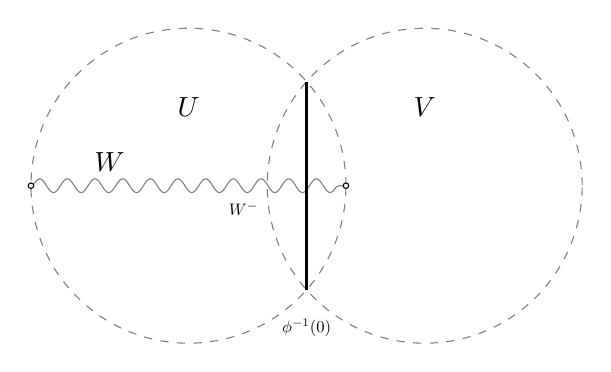
\begin{tikzpicture}
	\draw[gray, dashed] (0,0) circle (2);
	\node at (0,1){$U$};
	\draw[gray, dashed] (3,0) circle (2);
	\node at (3,1){$V$};
	\draw[gray, snake it] (-2,0) -- (2,0);
	\draw[black, fill=white] (-2,0) circle (1pt);
	\draw[black, fill=white] (2,0) circle (1pt);
	\draw[thick] (1.5, 1.32) -- (1.5, -1.32);
	\node[scale=.6] at (1.5, -1.8){$\phi^{-1}(0)$};
	\node[scale=.6] at (.7, -.3){$W^-$};
	\node[scale=1] at (-1, .3){$W$};
	\end{tikzpicture}
\end{document}
		\caption{For a proper map $r_W \colon W \to U$, the restriction to $W^-$ is proper into $U \cup V$.}
		\label{F: MV2}
	\end{figure}

	Finally, we also note that $\phi^{-1}(0)$ is closed in $U \cap V$, $U$, $V$, and $U \cup V$, so for any $W$ in $PC_\Gamma^*(-)$ for any of these spaces, $W^0$ is also in $PC^*_\Gamma(-)$ for all these spaces.

	These observations will be used freely in the remainder of the proof.

	\textbf{Exactness at $H^k_\Gamma(U \cup V)$.}
	Let $\uW \in H^{k-1}(U \cap V)$.
	Then $i\delta(\uW)$ is represented by $(-W^0, W^0)$.
	By the above discussion, we have $W^+ \in PC^*_\Gamma(U)$, and by applying the same discussion to $\bd (W^+)$ we also have in $U$ that $\bd (W^+) = W^0+(\bd W)^+$ via \cref{E: codim 1 pullbacks}.
	But $(\bd W)^+ \in Q^*(U)$ by \cref{C: creasing Q} as $W$ is a cocycle.
	Thus $W^0$ represents $0 \in H^k_\Gamma(U)$.
	Similarly, $W^0$ represents $0 \in H^k_\Gamma(V)$ using $W^-$.
	So $i\delta = 0$.

	Next suppose $\uW \in H^k_\Gamma(U \cup V)$ with $i(\uW) = 0$.
	Representing $\uW$ by $W$, this means that $W|_U$ and $W|_V$ each bound, in $U$ and $V$ respectively.
	This means there exist $A \in PC^*_\Gamma(U)$ and $S \in Q^*(U)$ with $\bd A = W|_U+S$ and $B \in PC^*_\Gamma(V)$ and $T \in Q^*(V)$ with $\bd B = W|_V+T$.
	We choose a common separating point for $A$ and $B$ and consider $A^-$ and $B^+$, which are both well defined in $U \cup V$ by the discussion above.
	We compute
	\begin{align*}
		\bd(A^-+B^+)& = -A^0 + (\bd A)^- +B^0+ (\bd B)^+\\
		& = -A^0 + (W|_U)^-+S^- +B^0+ (W|_V)^++T^+.
	\end{align*}
	But $(W|_U)^- +(W|_V)^+ = W^-+W^+$, which through the creasing construction is cohomologous to $W$.
	Further, $S^-+T^+ \in Q^*(U \cup V)$, so we see that $W$ is cohomologous to $A^0-B^0$.
	But $A^0-B^0 = \delta(B|_{U \cap V}-A|_{U \cap V})$.

	\textbf{Exactness at $H^k_\Gamma(U) \oplus H^k_\Gamma(V)$.}
	It is immediate that the composition $ji = 0$.

	Now suppose $(\uW_1,\uW_2) \in \ker j \subset H^k_\Gamma(U) \oplus H^k_\Gamma(V)$.
	Using representatives $W_1,W_2$, this means that there is a $Z \in C^k_\Gamma(U \cap V)$ with $\bd Z = W_1|_{U \cap V}+W_2|_{U \cap V}+T$, with $T \in Q^*(U \cap V)$.
	Choose a separating point for all $Z$ and hence automatically $W_1$, $W_2$, and $T$.
	We claim that $\gamma = W_1^- - Z^0 -W_2^+$ represents an element of $H^k_\Gamma(U \cup V)$ whose image under $i$ is $(\uW_1,\uW_2)$.
	We compute
	\begin{align*}\bd \gamma& = \bd (W_1^- - Z^0 -W_2^+)\\
		& = -W_1^0 +(\bd W_1)^- + (\bd Z)^0 - W_2^0 - (\bd W_2)^+\\
		& = -W_1^0 +(\bd W_1)^- + W_1^0+W_2^0+T^0 - W_2^0 - (\bd W_2)^+\\
		& = (\bd W_1)^- +T^0 - (\bd W_2)^+.
	\end{align*}
	As $W_1$ and $W_2$ are cycles, $(\bd W_1)^-$, $(\bd W_2)^+$, and $T^0$ are in $Q^*(U \cup V)$.
	So this boundary is $0$ in $C^*_\Gamma(U \cup V)$, and $\gamma$ represents an element of $H^k_\Gamma(U \cup V)$.

	Next we show that $\gamma|_U$ is cohomologous to $W_1$ in $U$.
	In fact, in $U$ we have
	$$\bd (Z^+) = Z^0+(\bd Z)^+ = Z^0+ W_1^++ W_2^+|_{U}+T^+.$$ So
	$\bd (Z^+) +\gamma|_U = W_1^-+W_1^+ +T^+$, and we see that $\gamma|_U$ is cohomologous in $U$ to $W_1^-+W_1^+$, which is cohomologous to $W_1$ in $U$ via creasing.
	Similarly, in $V$ we have
	$$\bd (Z^-) = -Z^0+(\bd Z)^- = -Z^0+W_1^-|_{V}+ W_2^-+T^-.$$
	So
	$\bd(Z^-) - \gamma|_V = W_2^-+W_2^+ +T^-$, and $-\gamma|_V$ is cohomologous to $W_2^-+W_2^+$, which is cohomologous to $W_2$ in $V$.

	So $(\uW_1,\uW_2) = i(\underline{\gamma})$.

	\textbf{Exactness at $H^k_\Gamma(U \cap V)$.}
	Consider a cocycle $W$ in $C^k_\Gamma(U)$.
	Then $\delta j(\uW)$ is represented by $-W^0$.
	By the discussion above, $W^- \in PC^*_\Gamma(U \cup V)$, and $$\bd (W^-) = -W^0+ (\bd W)^-.$$ As $W$ is a cocycle, $\bd W \in Q^*(U)$, and so $(\bd W)^- \in Q^*(U \cup V)$ via \cref{C: creasing Q}.
	So $\delta j(\uW) = 0 \in H^*_\Gamma(U \cup V)$, and similarly for elements of $H^k_\Gamma(V)$.

	Now suppose $\uW \in H^k_\Gamma(U \cap V)$ and $\delta(\uW) = 0$.
	Representing $\uW$ by $W$ and choosing a separating function and separating point, this means there is a $Z$ in $U \cup V$ such that $\bd Z = -W^0+T$ with $T \in Q^*(U \cup V)$.
	Let $A = Z|_U+ W^+ \in PC^*_\Gamma(U)$ and $B = -Z|_V +W^- \in PC^*_\Gamma(V)$.
	Then
	\begin{align*}
		\bd A& = \phantom{-}\bd Z|_U+ \bd( W^+) = -W^0+T|_U +W^0+(\bd W)^{+} = \phantom{-}T|_U+(\bd W)^{+}\\
		\bd B& = -\bd Z|_V+ \bd (W^-) = \phantom{-}W^0-T|_V -W^0+(\bd W)^{-} = -T|_V+(\bd W)^{-}.
	\end{align*}
	As $\bd W \in Q^*(U \cap V)$ and $T \in Q^*(U \cup V)$, their pullbacks and restrictions are also in the appropriate $Q^*$s, so $(A,B)$ represents an element of $H^k_\Gamma(U) \oplus H^k_\Gamma(V)$.

	We then have
	\begin{align*}
		j(A,B)& = A|_{U \cap V}+B|_{U \cap B}\\
		& = Z|_{U \cap V}+ W^+ - Z|_{U \cap V} +W^-\\
		& = W^++W^-,
	\end{align*}
	which represents $\uW \in H^k(U \cap V)$ via creasing.
\end{proof}

\begin{comment}

	\subsection{The suspension map and the cohomology of Euclidean space}\label{S: suspension}

	\red{I'm leaving it for now, but I'm not sure we need this section anymore (which is a shame as I enjoyed writing it).}

	\begin{proposition}
		$H_\Gamma^*(\R^n) \cong H^*(\R^n)$.
	\end{proposition}

	The proof of the proposition will proceed by an induction over the dimension $n$.
	For $n = 0$, the domains of all cochains must be compact and oriented, so $H^*_\Gamma(\R^0) = H_*^\Gamma(\R^0)$, where the latter represents Lipyanskiy's geometric homology theory, which is isomorphic to singular homology by \cite[Section 10]{Lipy14} (or in this case by direct computation).
	For $n>0$, our general strategy will be derived from the treatment of non-compactly supported piecewise-linear intersection homology in \cite[Section II.2]{BoHab}.
	In particular, we have the following two lemmas modifying \cite[Lemmas 2.2 and 2.3]{BoHab}.

	\begin{lemma}
		Let $M$ be a manifold, and suppose $\uW \in C^{i}_\Gamma(\R \times M)$ is a cocycle with support in $\R_+ \times M$.
		Then $\uW$ is the coboundary of a cochain in $C^{i-1}_\Gamma(\R \times M)$ supported in $\R_+ \times M$.
	\end{lemma}
	\begin{proof}
		Let $p_1 \colon \R \times M \to \R$ and $p_2 \colon \R \times M \to M$ be the projections, and let $r_W \colon W \to \R_+ \times M$ be the reference map.
		Note that $\R_+ \times W$ is a manifold with corners by \cite[Theorem 6.4]{Joy12}.
		So we can define a new map $r_{\R_+ \times W} \colon \R_+ \times W \to \R \times M$ by $r_{\R_+ \times W}(t,x) = (t+p_1r_W(x),p_2r_W(x))$.
		As $r_W$ is proper, so is $r_{\R_+ \times W}$, and its boundary (up to signs) is the sum of $W$ with $\pm r_{\R_+ \times \bd W} \colon \R_+ \times \bd W \to \R \times M$, letting this latter map be constructed analogously to $r_{\R_+ \times W}$.
		As $\bd W$ represents $0$ in $C^*_\Gamma(\R \times W)$, it must be a sum of trivial and degenerate objects.
		But it is easy to see that our construction takes trivial and degenerate objects to trivial and degenerate objects, respectively, so that $\R_+ \times \bd W$ is a sum of trivial and degenerate objects.
		Thus $W$ cobounds as required.
	\end{proof}

	In this section we give an explicit construction of the cohomology suspension isomorphism

	\begin{proposition}[Suspension isomorphism]
		Define the suspension map\footnote{Note that the suspension map $S$ has degree $0$ as the degree of an element of $W$ is determined by the codimension $\dim(M)-\dim(W)$, which is preserved under suspension.
		} $S:PC^*_\Gamma(M) \to PC^{*}_\Gamma(\R \times M)$ so that if $W \in PC^*_\Gamma(M)$ is represented by $r_W \colon W \to M$ then $S(W)$ is represented by $r_{\R \times W} \colon \R \times W \to \R \times M$ defined by $r_{\R \times W}(t,x) = (t,r_W(x))$.
		Then $S$ induces isomorphisms $S \colon H^*_\Gamma(M) \to H^{*}_\Gamma(M)$.
	\end{proposition}
	\begin{proof}
		We first observe that $S$ descends to a well-defined map $C^*_\Gamma(M) \to C^{*}_\Gamma(\R \times M)$, as it is easy to see that it preserves the properties of being trivial or degenerate.
		It is also clearly a chain map.

		Next, we note that $S: C^*_\Gamma(M) \to C^{*}_\Gamma(M)$ is injective: In order for $\R \times W$ to be trivial, each $\{t\} \times W$ would have to be trivial so that $W$ would be trivial, and similarly in order for $\R \times W$ to be degenerate, $W$ would have to be degenerate.
		Thus it suffices to show that the quotient of $C^{*}_\Gamma(M)$ by the image of $C^*_\Gamma(M)$ is acyclic.
		To do so, we must show that if $\uW \in C^{*}_\Gamma(M)$ and $\bd W = S(V)+T$ for some $V \in PC^*_\Gamma(M)$ and $T \in Q^*(M)$ then $W = \bd Z+S(V')+T'$ for some $V' \in PC^*_\Gamma(M)$ and $T' \in Q^*(M)$.

		Consider the map $p \colon \R \times M \to \R$.
		The composite $pr_W$ must have a regular value by Sard's theorem; without loss of generality, we assume this is at $0$.
		As in the creasing construction, let $W_0 = (pr_W)^{-1}(0)$, $W^+ = (pr_W)^{-1}([0,\infty))$, and $W^- = (pr_W)^{-1}((-\infty,0])$.
		We can also think of these as the pullbacks $p^{-1}(0) \times_M W$, etc.
		Similarly, we consider $S(W_0)$ and note that it has an analogous creasing decomposition with $(S(W_0))_0 = W_0$, $S(W_0)^+ = \R_+ \times W_0$, and $S(W_0)^- = \R_- \times W_0$.
		We will also need to consider $\bd (W_0)$.
		From the properties of pullbacks \cite[Proposition 7.4]{Joy12} (from which we get the sign in the following formula using that $W_0 = p^{-1}(0) \times_M W$), we have
		$$\bd(W_0) = -(\bd W)_0 = -S(V+T)_0 = -S(V)_0-T_0 = -V-T_0.$$

		%p^{-1}((-infty,0]) \times_M W

		Next, we consider $W^--(\R_- \times W_0)$.
		Its boundary, again using the sign conventions from Joyce, is
		\begin{align*}
			\bd (W^--(\R_- \times W_0))& = \bd(W^-)-\bd (\R_- \times W_0) \\
			& = [W_0+(S(V)+T)^- ]-[W_0-\R_- \times \bd W_0]\\
			& = (\R_- \times V)+T^-+(\R_- \times \bd W_0)\\
			& = (\R_- \times V)+T^-+(\R_- \times (-V-T_0))\\
			& = (\R_- \times V)+T^--(\R_- \times V)-(\R_- \times T_0)\\
			& = T^--(\R_- \times T_0).
		\end{align*}
		As $T$ is an element of $Q^*(\R \times M)$ and $T^-$ and $T_0$ are pullbacks of $T$ with other precochains, they are also in $Q^*(\R \times M)$ by REF.
		It follows that $\R_- \times T_0$ is also in $Q^*(\R \times M)$, so
		$W^--(\R_- \times W_0)$ is a cocycle in $C_\Gamma^*(\R \times M)$ that is supported in $\R_- \times M$.
		By the preceding lemma, it cobounds, i.e.\ there is a $Z_1$ with $\bd Z_1 = W^--(\R_- \times W_0)+A_1$, with $A_1 \in Q^*(\R \times M)$.

		Analogously, there are $Z_2$ and $A_2$ such that $\bd Z_2 = W^+-(\R_+ \times W_0)+A_2$.

		We now consider the cochain $\Cre(W)-\Cre(S(W_0))-Z_1-Z_2$.
		Its boundary is
		\begin{align*}
			\bd(\Cre(W)&-\Cre(S(W_0))-Z_1-Z_2)\\
			& = W^++W^--W-\Cre(\bd W)-[(\R_+ \times W_0)+(\R_- \times W_0)-S(W_0)-\Cre(\bd S(W_0))] \\
			&\phantom{ = } -W^-+(\R_- \times W_0)-A_1-W^++(\R_+ \times W_0)-A_2\\
			& = -W+S(W_0)-\Cre(\bd W)+\Cre(\bd S(W_0))-A_1-A_2
		\end{align*}

		Now recall that $\bd W = S(V)+T$, while $\bd S(W_0) = \bd(\R \times W_0) = -\R \times \bd W_0 = -S(\bd W_0) = -S(-V-T_0) = S(V+T_0)$.
		So $\Cre(\bd W)-\Cre(\bd S(W_0)) = \Cre(T)-\Cre(S(T_0))$.
		We already know $A_1,A_2 \in Q^*(\R \times M)$.
		Furthermore, $\Cre(T), \Cre(S(T_0)) \in Q^*(\R \times M)$ as we have noted that the suspension of an element of $Q^*(M)$ is in $Q^*(\R \times M)$ and the creasing of an element of $Q^*(\R \times M)$ is in $Q^*(\R \times M)$ by the proof of \cite[Lemma 18]{Lipy14}.

		So, we have established a cohomology between $W$ and $S(W_0)$ as desired.
	\end{proof}
\end{comment}

\subsection{Geometric homology and cohomology are singular homology and cohomology}\label{S: homology is homology}

In this section we apply a theorem of Kreck and Singhof to show that geometric homology and cohomology are isomorphic to singular homology and cohomology on smooth manifolds.

\begin{theorem}\label{T: geometric is singular}
	On the category of smooth manifolds (without boundary) and continuous maps, geometric homology and cohomology are respectively isomorphic to singular homology and cohomology with integer coefficients, i.e.\ $H_*^\Gamma \cong H_*(\cdot ;\Z)$ and $H^*_\Gamma \cong H^*(\cdot ;\Z)$ as functors.
\end{theorem}

\begin{proof}
	This is a consequence of \cite[Theorem 10]{Krec10b} once we verify that $H_*^\Gamma$ and $H^*_\Gamma$ are respectively an ordinary homology theory and an ordinary cohomology theory on the category of smooth manifolds as defined in \cite{Krec10b}.
	This requires the following axioms:

	\begin{enumerate}
		\item\label{I: homotopy functor} $H_*^\Gamma$ is a covariant functor on the category of smooth manifolds (without boundary) and continuous maps between them, and $H^*_\Gamma$ is a contravariant homotopy functor on the same category.

		\item For each triple $(M;U,V)$ with $M$ a smooth manifold and $U,V$ open subsets such that $U \cup V = M$ there are exact (homological or cohomological) Mayer--Vietoris sequences with natural connecting maps $\delta$.

		\item\label{I: neg dim} For all $M$, $H_k^\Gamma(M) = H^k_\Gamma(M) = 0$ for $k<0$.

		\item The Dimension Axiom: $H_k^\Gamma(pt) = H^k_\Gamma(pt) = 0$ for $k\neq 0$ and $H^\Gamma_0(pt) \cong H_\Gamma^0(pt) \cong \Z$.

		\item $H_*^\Gamma$ and $H^*_\Gamma$ are additive: for a manifold $M$ of dimension $0$, each $H_k^\Gamma(M)$ is canonically isomorphic to $\oplus_{x \in M} H_k^\Gamma(x)$ and each $H^k_\Gamma(M)$ is canonically isomorphic to $\prod_{x \in M} H^k_\Gamma(x)$.
	\end{enumerate}

	Axiom \ref{I: homotopy functor} holds from the definitions and \cref{P: homology homotopy functor,P: cohomology pullback}.
	We have Mayer--Vietoris sequences by \cref{T: relative MV,T: absolute MV}.
	The connecting map for the cohomology sequence is natural by \cref{L: natural connection}.
	The connecting map for the homology sequence is natural just as in the standard argument for singular homology: given a map of triples $(M;U',V') \to (N;U,V)$ there is a map of Mayer--Vietoris sequences induced by a map of short exactly sequences of chain complexes of the form of diagram \eqref{E: homology MV SES} (replacing supported cochains complexes with chain complexes), itself induced by functoriality from the maps of chain complexes $C_*^{\Gamma}(U') \to C_*^{\Gamma}(U)$ and similarly for $V$ and $U \cap V$.
	This map of Mayer--Vietoris sequences in particular shows that the connecting map is natural.

	Axiom \ref{I: neg dim} holds trivially for homology as there are no chains of degree $<0$.
	It also holds for cohomology because for $k<0$ any representing cocycle must have small rank and boundary in $Q^*(M)$.
	Thus any such cocycle must be $0 \in C^k_\Gamma(M)$.

	The Dimension Axiom has been proven in \cref{E: dimension}.

	The Additivity Axiom is apparent.
\end{proof}

\begin{example}
	Let us consider $H^*_\Gamma(\R P^2)$.
	We know from the standard computations of $H^*(\R P^2)$ and the above theorem that
	\begin{equation*}
		H_\Gamma^i(\R P^2) =
		\begin{cases}
			\Z_2,&i = 2,\\
			\Z,&i = 0,\\
			0,&\text{otherwise.}
		\end{cases}
	\end{equation*}
	From the viewpoint of geometric cohomology, $H^0(\R P^2)$ is generated by the identity map $\R P^2 \to \R P^2$, which is co-oriented at each point by $(\beta,\beta)$ for any local orientation $\beta$.

	In degree $1$, cochains are represented by co-oriented maps from (unions of) closed intervals or circles.
	For a map from the circle to be co-oriented it cannot represent the non-trivial element $\alpha \in \pi_1(\R P^2)$, and so it must be contractible.
	Any map from a disk must be co-orientable, as the disk is contractible (this can be considered an extension of \cref{L: co-orientable homotopies}).
	Thus by smooth approximation, any smooth co-oriented map from the circle to $\R P^2$ is the boundary of a smooth co-oriented map from the disk, and so represents $0$ in cohomology.
	The same is true for any ``circle of intervals'' that does not represent $\alpha \in \pi_2(\R P^2)$; via homotopy and creasing, such a ``circle'' is the boundary of a polygon.
	On the other hand, consider a map $g \colon \interval \to \R P^2$ that does represent $\alpha$.
	As $\interval$ is contractible, such a map can always be co-oriented.
	We can let $e$ represent the standard unit vector of $\interval$ and suppose that $g$ is co-oriented so that at $0 \in \interval$ the co-orientation is represented by $(e,\beta)$ for some local orientation $\beta$ of $\R P^2$ at $f(0)$.
	Traversing the path, the representation for the co-orientation at $1$ is then $(e,-\beta)$.
	Recalling our boundary conventions, the boundary of $f$ therefore consists of the maps $f|_0:0 \to \R P^2$ co-oriented by $(1,e)*(e,\beta) = (e,\beta)$ and $f|_1:1 \to \R P^2$ co-oriented by $(1,-e)*(e,-\beta) = (e,\beta)$.
	Thus with these co-orientations, $f|_0:0 \to \R P^2$ and $f|_1:1 \to \R P^2$ represent isomorphic manifolds over $\R P^2$.
	As a co-oriented map from any single point to $\R P^2$ is a cocycle, we see by choosing the image to be the basepoint for $\pi_1(\R P^2)$ that twice any such map is a boundary.
	We leave it to the reader to verify that any two such points generate the same cohomology class, and so we have verified that $H^1_\Gamma(\R P^2) = 0$ and $H_\Gamma^2(\R P^2) \cong \Z_2$.
\end{example}

\subsubsection{A more direct comparison of singular and geometric homology}

While it was convenient to cite simultaneously the homology and cohomology versions of the Kreck-Singhof theorem, we can provide a second proof in the homology case that says a bit more.
In particular, as simplices are manifolds with corners and as the standard model simplex comes equipped with an orientation, if we let $S^{sm}_*(M)$ denote the chain complex of smooth singular chains, there is an obvious inclusion map $S^{sm}_*(M) \into PC_*^\Gamma(M)$.
It is not hard to check consistency of the boundary orientations so that this induces a chain map $S^{sm}_*(M) \to C_*^\Gamma(M)$.
We will see that this is a quasi-isomorphism.
Combined with the well-known fact that the inclusion $S^{sm}_*(M) \into S_*(M)$ is a chain homotopy equivalence if $S_*(M)$ is the full singular chain complex on $M$ \cite[Theorem 18.7]{Lee13}, this provides a concrete chain of isomorphisms $H_*(M) \cong H_*^\Gamma(M)$.

It will also be useful below to have the analogous result for cubical singular homology in addition to the more common simplicial singular homology.
Details of cubical singular homology can be found, for example, in (see, e.g., \cite{Mas91} or \cite[Section 8.3]{HW60}).
Rather than maps of simplices $\Delta^k \to M$, the cubical singular chain complex $SK_*(M)$ is generated by maps $\interval^k \to M$ with $\interval$ being the standard interval $\interval = [0,1]$.
The boundary formula is defined so that if $\sigma: \interval^k \to M$ is a singular cube, then
\begin{equation}\label{E: cube bd}
	\bd \sigma = \sum_{i = 1}^k (-1)^i(\sigma \delta_i^0-\sigma \delta^1_i),
\end{equation}
where for $\epsilon\in\{0,1\}$, the map $\delta_i^\epsilon \colon \interval^{k-1} \to \interval^k$ is defined by
$$\delta_i^\epsilon(x_1,\ldots,x_k) = (x_1,\ldots,\epsilon,\ldots, x_k)$$
with $\epsilon$ in the $i$th slot.
The homology of the chain complex $SK_*(M)$ is not isomorphic to singular homology as it does not satisfy the dimension axiom, so one instead forms the normalized complex $NK_*(M)$ by quotienting out the subcomplex of degenerate singular cubes, generated by singular cubes $\sigma \colon \interval^k \to M$ such that $\sigma$ does not depend on at least one of the variables.
In other words, the degenerate singular cubes are those maps $\sigma \colon \interval^k \to M$ that factor through one of the standard projections $\interval^k \to \interval^{k-1}$.
It then holds that $NK_*(M)$ is chain homotopy equivalent to $S_*(M)$.
In fact this holds for $M$ any space and not just a manifold \cite[Theorem 8.4.7]{HW60}.
Of course we will need the smooth version $NK^{sm}_*(M)$ generated by smooth singular cubes and modulo degenerate smooth singular cubes.
We defer to an appendix to this section the proof that $NK^{sm}_*(M) \into NK_*(M)$ is a chain homotopy equivalence.

As the cubes $\interval^k$ are compact manifolds with corners equipped with their standard orientations,
we have inclusion $SK^{sm}_i(M) \into PC_i^\Gamma(M)$ for all $i$.

\begin{lemma}
	The inclusion $SK^{sm}_*(M) \into PC_*^\Gamma(M)$ determines a chain map $NK^{sm}_*(M) \to C_*^\Gamma(M)$.
\end{lemma}

\begin{proof}
	Any degenerate singular cube $\sigma \colon \interval^k \to M$ is also degenerate in the sense of \cref{D: equiv triv and small}.
	In fact, it will have small rank as it filters through a projection.
	Furthermore, if that projection collapses the $i$th coordinate then each face $\sigma \delta_j^\epsilon$ for $j\neq i$ will also be a degenerate small cube and so have small rank, while the term $\pm (\sigma \delta_i^0-\sigma \delta_i^1)$ will be trivial with the trivializing map $\rho$ being the interchange of the two faces.
	Thus, the degenerate smooth singular cubes are elements of $Q_*(M)$, and our map is well defined in each degree.

	We check compatibility of boundary orientations.
	Consider the $n-1$ face $F$ of $\interval^n$ given by $x_i = j$ with $j\in\{0,1\}$.
	Then we have an outward pointing vector given by $(-1)^{j+1}e_i$, where $e_i$ is the vector in the positive $i$th direction.
	In general if we let $\beta_k$ denote the positive orientation corresponding to the $k$th coordinate, then the boundary orientation for $\beta_F$ is the one such that
	$(-1)^{j+1}\beta_i \wedge \beta_F$ is the orientation $\beta_1 \wedge\cdots\wedge \beta_n$ of $\interval^n$.
	Thus the boundary orientation is $(-1)^{j+1+i-1}\beta_1 \wedge \cdots \wedge \hat{\beta}_i \wedge \cdots\beta_n$.
	On the other hand, $\beta_1 \wedge \cdots \wedge \hat{\beta}_i \wedge \cdots\beta_n$ is precisely the standard orientation of $F$ when considering $\interval^n$ as a cubical complex.
	So the boundary orientation of $F$ is $(-1)^{i+j}$ times its orientation in the cubical complex.
	But this corresponds precisely to the formula for the boundary in $K^{sm}_*(M)$ coming from equation \eqref{E: cube bd}.
\end{proof}

\begin{comment}
	As the cubes $\interval^k$ are compact manifolds with corners equipped with their standard orientations,
	we have $SK^{sm}_*(M) \into PC_*^\Gamma$.
	Furthermore, any degenerate singular cube $\sigma \colon \interval^k \to M$ is also degenerate in the sense of Definition \ref{D: equiv triv and small}.
	In fact, it will have small rank as it filters through a projection.
	Furthermore, if that projection collapses the $i$th coordinate then each face $\sigma \delta_j^\epsilon$ for $j\neq i$ will also be a degenerate small cube and so have small rank, while the term $\pm (\sigma \delta_i^0-\sigma \delta_i^1)$ will be trivial with the trivializing map $\rho$ being the interchange of the two faces.
	Thus, the degenerate smooth singular cubes are elements of $Q_*(M)$.
	As in the simplicial case one can check compatibility of boundary orientations so that we have a chain map $NK^{sm}_*(M) \to C_*^\Gamma(M)$.
	\red{NEED TO PROVE THIS IS A CHAIN MAP}
\end{comment}

\begin{theorem}\label{T: hom iso map}
	The maps $H_*(S^{sm}_*(M)) \to H_*^\Gamma(M)$ and $H_*(NK^{sm}_*(M)) \to H_*^\Gamma(M)$ obtained by treating smooth singular simplices and smooth singular cubes as elements of $C_*^\Gamma(M)$ are isomorphisms.
\end{theorem}

\begin{proof}
	Both $H_*(S^{sm}_*(M))$ and $H_*(NK^{sm}_*(M))$ are isomorphic to the standard singular homology groups, so in the following we simply write $H_*$ for either of these theories and provide a uniform proof.

	We apply Theorem \cite[5.1.1]{Frie20}, which is based on standard Mayer--Vietoris techniques.
	In particular, on the category consisting of the open sets of $M$, the maps $\Phi: H_*(-) \to H_*^\Gamma(-)$ provide a natural transformation of functors.
	We need to check the following three properties:

	1.
	On $\emptyset$ or $U \subset M$ with $U$ homeomorphic to $\R^m$, the map $\Phi: H_*(U) \to H_*^\Gamma(U)$ is an isomorphism.
	As both $H_*$ and $H_*^\Gamma(-)$ are homotopy functors, we know from the respective Dimension Axioms (see \cref{E: dimension}) that in this case $H_k(U) = H_k^\Gamma(U) = 0$ for $k\neq 0$, while for $k = 0$ we have the commutative diagram
	\[
	\begin{tikzcd}
		H_0(pt) \arrow[r] \arrow[d, "\Phi"] & H_0(U) \arrow[d, "\Phi"] \\
		H_0^\Gamma(pt) \arrow[r] & H^\Gamma_0(U).
	\end{tikzcd}
	\]
	The horizontal maps are isomorphisms because these are homotopy functors, and the left hand vertical map is an isomorphism because $\Phi$ takes a generator of $H_0(pt) \cong \Z$ to a generator of $H_0^\Gamma(pt) \cong \Z$; see again \cref{E: dimension}.
	So the right hand map is also an isomorphism.

	2.
	$\Phi$ induces a commutative diagram of long exact Mayer--Vietoris sequences.
	This follows from basic homological algebra given the commutativity of the following diagram and its analogue for singular cubical chains
	\[
	\begin{tikzcd}[column sep=large]
		S_*(U \cap V) \arrow[r, "{(i_U, -i_V)}", hook] \arrow[d, "\Phi"] & S_*(U) \oplus S_*(V) \arrow[d, "\Phi \oplus \Phi"] \\
		C_*^\Gamma(U \cap V) \arrow[r, "{(i_U, -i_V)}", hook] & C_*^\Gamma(U) \oplus C_*^\Gamma(V).
	\end{tikzcd}
	\]

	3.
	If $\{U_\alpha\}$ is an increasing collection of open submanifolds of $M$ such that $\Phi \colon H_*(U_\alpha) \to H_*^\Gamma(U_\alpha)$ is an isomorphism for all $\alpha$, then $\Phi \colon H_*(\cup_\alpha U_\alpha) \to H_*^\Gamma(\cup_\alpha U_\alpha)$ is an isomorphism.
	This argument is standard given that both singular (simplicial or cubical) chains and geometric chains are represented by compact spaces: If $W$ represents a cycle in $C_*^\Gamma(\cup_\alpha U_\alpha)$, then $W \to \cup_\alpha U_\alpha$ factors through some particular $U_\beta$, so, as $H_*(U_\beta) \xr{\Phi}H_*^\Gamma(U_\beta)$ is an isomorphism, $\uW$ is in the image of $H_*(U_\beta) \xr{\Phi}H_*^\Gamma(U_\beta) \to H_*^\Gamma(\cup_\alpha U_\alpha)$.
	But then $\uW$ is in the image of composition $H_*(U_\beta) \to H_*(\cup_\alpha U_\alpha) \to H_*^\Gamma(\cup_\alpha U_\alpha)$, so $\Phi \colon H_*(\cup_\alpha U_\alpha) \to H_*^\Gamma(\cup_\alpha U_\alpha)$ is surjective.
	Similarly, if $\Phi \colon H_*(\cup_\alpha U_\alpha) \to H_*^\Gamma(\cup_\alpha U_\alpha)$ maps a class represented by a singular cycle $\xi$ to $0$, then $\xi$ bounds as a geometric cycle, say $\bd W = \xi+T$ for some $T \in Q_*(U)$.
	But by compactness, there is some $\beta$ so that $W$, $T$, and $\xi$ all have image in $U_\beta$.
	So $\xi$ represents a class in $H_*(U_\beta)$ that maps to $0$ in $H_*^\Gamma(U_\beta)$.
	As $\Phi$ is assumed an isomorphism on $U_\beta$, it must be that $\xi$ represents $0$ in $H_*(U_\beta)$, and so it also represents $0$ in $H_*(\cup_\alpha U_\alpha)$.

	It now follows from Theorem \cite[5.1.1]{Frie20} that $\Phi: H_*(M) \to H_*^\Gamma(M)$ is an isomorphism.
\end{proof}

\cref{T: hom iso map} is claimed without proof in \cite[Section 10]{Lipy14}.
Lipyanskiy states ``The fact that the natural maps induce isomorphisms follow from the standard Mayer--Vietoris arguments.'' However, these arguments are not given and, in fact, no Mayer--Vietoris sequence is proven to exist in \cite{Lipy14}, though the main required tool, creasing, is provided.

Unfortunately, providing a direct comparison for cohomology theories is not so straight forward as there is no obvious map between $C^*_\Gamma(M)$ and $S^*(M) = \Hom(S_*(M),\Z)$.
It will take some work in the following sections to develop a geometric connection between these cohomology theories.

\subsection{Appendix: smooth singular cubes}

\begin{proposition}\label{P: singular smooth cubes}
	The inclusion $\psi: NK^{sm}_*(M) \into NK_*(M)$ is a chain homotopy equivalence.
\end{proposition}

\begin{proof}
	The proof is analogous to the simplicial case as given in detail in \cite[Theorem 18.7]{Lee13}, though we need to take care with degenerate cubes, which is not an issue in the simplicial case.
	To account for this, we sketch the proof in \cite{Lee13} but provide some detailed modifications.

	We first observe that the map $SK^{sm}_*(M) \to NK_*(M)$ takes a smooth singular cubical chain to $0$ only if all of its cubes (with non-zero coefficient) are degenerate, and so we do have an injection $NK^{sm}_*(M) \into NK_*(M)$.
	We will define cube-wise a chain homotopy inverse $s \colon NK_*(M) \to NK^{sm}_*(M)$ by starting with a map $\td s \colon SK_*(M) \to SK^{sm}_*(M)$ and passing to quotients.

	Recall from \cref{S: homology is homology} that we write $\delta_i^\epsilon$ for the face inclusions of the standard cubes.
	If $\sigma \colon \interval^k \to M$ is a singular cube, we define homotopies $H_\sigma \colon \interval^k \times \interval = \interval^{k+1} \to M$ so that the following properties hold:
	\begin{enumerate}
		\item\label{I: smooth} $H_\sigma$ is a homotopy from $\sigma$ to a smooth map $\td \sigma \colon \interval^k \to M$.

		\item\label{I: faces} $H_{\sigma \delta_i^\epsilon} = H_\sigma \circ (\delta_i^\epsilon \times \id_\interval)$ so that the construction is compatible along faces.
		More explicitly, $H_{\sigma \delta_i^\epsilon}(x,t) = H_\sigma(\delta_i^\epsilon(x),t)$.

		\item If $\sigma$ is smooth then $H_{\sigma}(x,t) = \sigma(x)$, i.e.\ the homotopy is constant.

		\item\label{I: degen} If $\sigma$ is independent of the coordinate $x_i$ then so is $H_\sigma$.
	\end{enumerate}

	The last condition, which we have added for cubes, ensures that if $\sigma$ is degenerate so will be $H_\sigma$ and $\td \sigma$.

	The construction is by induction on dimension.
	If $\sigma$ is a $0$-cube, then we define $H_\sigma(x,t) = \sigma(x)$, the constant homotopy.
	This satisfies the conditions.
	We then assume $H_\sigma$ defined with these properties for all cubes of dimension $<k$ and extend the definition to $k$-cubes.
	If $\sigma$ is already smooth, then the constant homotopy $H_\sigma(x,t) = \sigma(x)$ satisfies the conditions, noting that if $\sigma$ is smooth then so is each $\sigma \circ \delta_i^\epsilon$.
	If $\sigma$ is not smooth, we consider separately the two cases when $\sigma$ is degenerate or nondegenerate.

	First suppose $\sigma$ is not degenerate.
	By the induction hypothesis and Condition \eqref{I: faces}, $H_\sigma$ is determined on $(\interval^k \times 0) \cup (\bd \interval^k \times \interval)$.
	One can check as in the proof of \cite[Lemma 18.8]{Lee13} that Condition \eqref{I: faces} guarantees that the faces glue to form a continuous map.
	As $\bd \interval^k \into \interval^k$ is a cofibration, there is a retraction $\interval^k \times \interval \to (\interval^k \times 0) \cup (\bd \interval^k \times \interval)$, and the composition determines a homotopy $F \colon \interval^k \times \interval \to M$ such that $F(-,1)$ is smooth on each $k-1$ face of $\bd \interval^k$.
	In fact, this implies that $F(-,1)$ is smooth on all of $\bd \interval^k$ by a minor modification of \cite[Lemma 18.9]{Lee13}.
	So by the Whitney Approximation Theorem \cite[Theorem 6.26]{Lee13}, there is a homotopy rel $\bd \interval^k$ from $F(-,1)$ to a smooth map $\td \sigma \colon \interval^k \to M$; we denote this homotopy $G$.
	Finally, let $u \colon \interval^k \to (0,1]$ be a continuous function that takes $\bd\interval^k$ to $1$ and the interior of the cube to $(0,1)$.
	Then we can define
	\begin{equation*}
		H_\sigma(x,t) =
		\begin{cases}
			F\left(x,\frac{t}{u(x)}\right),&x \in \interval^k, 0 \leq t \leq u(x),\\
			G\left(x,\frac{t-u(x)}{1-u(x)}\right),&x \in \text{Int}(\interval^k), u(x) \leq t \leq 1.\\
		\end{cases}
	\end{equation*}
	One can check as in the proof of \cite[Lemma 18.8]{Lee13} that this is a continuous homotopy that satisfies the first two conditions above, as required.

	Next suppose $\sigma$ is degenerate, i.e.\ there is some coordinate $x_i$ so that $\sigma$ does not depend on $x_i$.
	Let $\pi_i \colon \interval^k\to\interval^{k-1}$ be given by $\pi_i(x_1,\ldots, x_k) = (x_1,\ldots, \hat x_i, \ldots, x_k)$ with the $x_i$ term omitted.
	In this case we let $H_\sigma(x,t) \defeq H_{\sigma \delta_i^0}(\pi_i(x),t) = H_{\sigma \delta_i^1}(\pi_i(x),t)$.
	We claim that if there are multiple coordinates of which $\sigma$ is independent then this definition is independent of the choice of such coordinate.
	This is clear for $1$-cubes for which there is only one possible coordinate.
	Suppose then the claim proven in dimensions $<k$ and that $\sigma \colon \interval^k \to M$ is independent of $x_i$ and $x_j$ with $j<i$.
	Since $\sigma$ is independent of $x_j$, so is $\sigma \circ \delta_i^0$, so inductively $H_{\sigma \delta_i^0}(\pi_i(x),t) = H_{\sigma \delta_i^0\delta_j^0}(\pi_j\pi_i(x),t)$.
	Similarly, using that the $i$th coordinate of the cube is the $i-1$-st coordinate of the $j$th faces, we have $H_{\sigma \delta_j^0}(\pi_j(x),t) = H_{\sigma \delta_j^0\delta_{i-1}^0}(\pi_{i-1}\pi_j(x),t)$.
	But $\delta_i^0\delta_j^0$ and $\delta_j^0\delta_{i-1}^0$ determine the same $k-2$ face of $\interval^k$, and $\pi_j\pi_i(x) = \pi_{i-1}\pi_j(x)$.
	So both constructions give the same $H_\sigma$.

	In this case, Conditions \eqref{I: smooth} and \eqref{I: degen} hold by construction and by induction.
	We must verify Condition \eqref{I: faces}.
	If $\sigma$ is independent of $x_i$, the condition is clear by construction for the faces $\sigma\delta_i^0$ and $\sigma\delta_i^1$.
	For $j\neq i$, first suppose $i<j$.
	As $\sigma$ is independent of $x_i$, so is $\sigma\delta^j_\epsilon$, so
	\begin{align*}
		H_{\sigma\delta_j^\epsilon}(x,t)& = H_{\sigma\delta_j^\epsilon \delta_i^0}(\pi_i(x),t)\\
		& = H_{\sigma \delta_i^0\delta^{j-1}_\epsilon}(\pi_i(x)),t)\\
		& = H_{\sigma \delta_i^0}(\delta_{j-1}^\epsilon\pi_i(x)),t)\\
		& = H_{\sigma \delta_i^0}(\pi_i(\delta_j^\epsilon(x)),t)\\
		& = H_\sigma(\delta_j^\epsilon(x),t).
	\end{align*}
	Here the first equality uses our definition of $H_{\sigma\delta_j^\epsilon}$ as $\sigma\delta_j^\epsilon$ is independent of $x_i$.
	The second equality is an identity for cubical face inclusions.
	The third is Condition \eqref{I: faces} for $H_{\sigma \delta_i^0}$, which holds by induction hypothesis.
	The fourth equality is another cubical identity, and the last is the definition of $H_\sigma$.

	Similarly, if $j<i$, then $\sigma\delta_j^\epsilon$ is independent of its $i-1$-st coordinate, and we compute analogously:

	\begin{align*}
		H_{\sigma\delta_j^\epsilon}(x,t)& = H_{\sigma\delta_j^\epsilon \delta_{i-1}^0}(\pi_{i-1}(x),t)\\
		& = H_{\sigma \delta_{i}^0\delta_{j}^\epsilon}(\pi_{i-1}(x)),t)\\
		& = H_{\sigma \delta_{i}^0}(\delta_{j}^\epsilon\pi_{i-1}(x)),t)\\
		& = H_{\sigma \delta_{i}^0}(\pi_{i}(\delta_j^\epsilon(x)),t)\\
		& = H_\sigma(\delta_j^\epsilon(x),t).
	\end{align*}

	This completes our construction of the homotopies $H_\sigma$.
	We can now define $\td s \colon SK_*(M) \to SK^{sm}_*(M)$ by $\td s(\sigma) = H_\sigma(-,1)$.
	Then if $\td \psi: SK_*^{sm}(M) \to SK_*(M)$ is the inclusion, we have by definition that $\td s \td \psi = \id$.
	We show that $\td\psi\td s$ is chain homotopic to the identity\footnote{Here, finally, is a step that is easier in the cubical setting as we do not need to subdivide prisms into simplices.}.
	Indeed, if $\sigma$ is a singular $k$-cube then treating $H_\sigma$ as a singular $k+1$ cube we have

	\begin{align*}
		\bd H_\sigma& = \sum_{i = 1}^{k+1} (-1)^i\left(H_\sigma \delta_i^0-H_\sigma \delta^1_i\right)\\
		& = \left(\sum_{i = 1}^{k} (-1)^i\left(H_\sigma (\delta_i^0 \times \id_\interval)-H_\sigma (\delta^1_i \times \id_\interval)\right)\right) +(-1)^{k+1}(H_\sigma(-,0)-H_\sigma(-,1))\\
		& = \left(\sum_{i = 1}^{k} (-1)^i\left(H_{\sigma \delta_i^0}-H_{\sigma\delta^1_i}\right)\right) +(-1)^{k+1}(\sigma(-)-\td \psi\td s(\sigma)).
	\end{align*}
	So if we define $\td J(\sigma) = (-1)^{k+1}H_\sigma$, we obtain
	\begin{align*}
		(-1)^{k+1}\bd \td J(\sigma)& = \left(\sum_{i = 1}^{k} (-1)^i\left( (-1)^k\td J(\sigma \delta_i^0)-(-1)^k\td J(\sigma\delta^1_i)\right)\right) +(-1)^{k+1}\left(\sigma(-)-\td \psi\td s(\sigma)\right)\\
		& = (-1)^k\td J(\bd \sigma)+(-1)^{k+1}(\sigma(-)-\td \psi\td s(\sigma)),
	\end{align*}
	so $$\bd \td J(\sigma)+\td J(\bd \sigma) = \sigma(-,0)-\td \psi\td s(\sigma),$$
	which shows that $\td \psi\td s$ is chain homotopic to the identity.

	Finally, we note that, by definition and construction, $\td \psi$, $\td s$, and $\td J$ all take degenerate simplices to degenerate simplices so that these descend to chain maps $\psi \colon NK_*^{sm}(M) \to NK_*(M)$ and $s \colon NK_*(M) \to NK_*^{sm}(M)$ with $s\psi = \id$ and a chain homotopy $J \colon NK_*(M) \to NK_{*+1}(M)$.
\end{proof}